\documentclass[10pt,letterpaper]{article}
\usepackage{rldmsubmit}

\usepackage{pslatex}
\usepackage{graphicx}
\usepackage{float}
\usepackage{amsmath}
\usepackage[hidelinks]{hyperref}
\usepackage[numbers,super]{natbib}

\title{Episodic memory facilitates flexible decision making via access to detailed events}

\author{
{\large \bf Jonathan Nicholas} \\
Department of Psychology \\
New York University \\
New York, NY 10003 \\
\texttt{jonathan.nicholas@nyu.edu} \\
\And
{\large \bf Marcelo G. Mattar} \\
Department of Psychology \\
New York University \\
New York, NY 10003 \\
\texttt{marcelo.mattar@nyu.edu}
}

\newcommand{\fix}{\marginpar{FIX}}
\newcommand{\new}{\marginpar{NEW}}

\begin{document}

\maketitle

\begin{abstract}

Our experiences contain countless details that may be important in the future, yet we rarely know which will matter and which won't. This uncertainty poses a difficult challenge for adaptive decision making, as failing to preserve relevant information can prevent us from making good choices later on. One solution to this challenge is to store detailed memories of individual experiences that can be flexibly accessed whenever their details become relevant. By allowing us to store and recall specific events in vivid detail, the human episodic memory system provides exactly this capacity. Yet whether and how this ability supports adaptive behavior is poorly understood. Here we aimed to determine whether people use detailed episodic memories to make decisions when future task demands are uncertain. We hypothesized that the episodic memory system's ability to store events in great detail allows us to reference any of these details if they later become relevant. We tested this hypothesis using a novel decision making task where participants encoded individual events with multiple features and later made decisions based on these features to maximize their earnings. Across four experiments (total n = 472), we found that participants referenced episodic memories during decisions in feature-rich environments, and that they did so specifically when it was unclear at encoding which features would be needed in the future. Overall, these findings reveal a fundamental adaptive function of episodic memory, showing how its rich representational capacity enables flexible decision making under uncertainty.

\textbf{Keywords:} 
decision making; episodic memory; incremental learning

\end{abstract}

\section{Introduction}

Humans possess the remarkable capacity to remember individual events from the past in high fidelity using our episodic memory system\cite{tulvingEpisodicSemanticMemory1972, eichenbaumHippocampusMechanismsDeclarative1999}. From merely a single exposure, we can recall complex experiences consisting of many different details --- the taste of a meal, the layout of a restaurant, the conversation around a dinner table --- even when it is unclear whether we will actually ever need any of this information again. Why do we maintain such detailed memories of past events?

One possible answer is that this ability is adaptive, because the aspects of an experience that will be relevant for future behavior are rarely apparent when they are first encountered. For instance, when deciding whether to visit a restaurant, you may need to recall details that weren't previously important during your prior meals there, such as whether the menu can accommodate your vegan friend or if the ambiance is appropriate for a work meeting. By storing detailed representations of past experiences, our episodic memory system can allow us to access any of these details if they ever become relevant in the future. In this way, episodic memory may enable flexible decision making by allowing us to repurpose our memories for novel goals.

Despite a long history of work on the adaptive role of episodic memory\cite{bartlettRememberingStudyExperimental1932, andersonHumanMemoryAdaptive1989, schacterMemoryDistortionAdaptive2011, shohamyDopamineAdaptiveMemory2010}, computational research has only recently started to characterize the advantages it can provide for decision making\cite{lengyelHippocampalContributionsControl2008, gershmanReinforcementLearningEpisodic2017, nagyInterplayEpisodicSemantic2025}. A key theme in this work is that the episodic memory system is poised to address several shortcomings faced by other forms of memory, particularly incremental learning, which aids decision making by allowing us to gradually estimate the value of different choice options over many repeated encounters\cite{rescorlaTheoryPavlovianConditioning1972, shohamyHabitsReinforcementLearning2014, knowltonNeostriatalHabitLearning1996, schultzNeuralSubstratePrediction1997, bayerMidbrainDopamineNeurons2005, shohamyRoleDopamineCognitive2005, zaghloulHumanSubstantiaNigra2009}. Importantly, incremental learning suffers from a well-known problem called the \textit{curse of dimensionality}, which arises because computational and memory demands rapidly scale with the richness of what must be learned\cite{suttonReinforcementLearningSecond2018}. For instance, when learning about choice options with multiple features, an agent capable of only incremental learning would need to track and update values for each independently.

One way humans may circumvent this issue is by selectively learning about only the most relevant features of experience while ignoring information about the rest\cite{wilsonInferringRelevanceChanging2012}. Using selective attention in this way can allow for efficient decisions in high-dimensional environments --- when a feature is deemed relevant, its value is tracked and incrementally updated, requiring only a simple retrieval at choice time. Such a strategy is highly effective under circumstances in which feature relevance can be reliably inferred, and people likely employ it when this is the case\cite{leongDynamicInteractionReinforcement2017, nivReinforcementLearningMultidimensional2015}. But environments like this are, in reality, rare. Further, augmenting incremental learning with selective attention enforces rigidity, ultimately harming future choices that may depend on features that were initially ignored. There are also fundamental limits to the number of features that can be reasonably attended to and tracked simultaneously\cite{millerMagicalNumberSeven1956}, making this strategy increasingly impractical in the real world. These limitations are precisely the types of problems that episodic memory's detailed representations are best equipped to address.

A separate but related challenge is that incremental learning is most successful when experiences are repeated, yet actual experiences are unlikely to be encountered more than a single time. Episodic memory, by contrast, allows us to encode and retrieve individual experiences, making it naturally suited to real world environments where experiences rarely repeat\cite{gershmanReinforcementLearningEpisodic2017}. Indeed, this capacity for one-shot learning has dominated research on episodic memory's role in decision making, where much work has demonstrated that humans can effectively guide their decisions by retrieving and leveraging individual past experiences\cite{bornsteinRemindersChoicesBias2017, duncanModulatingUseMultiple2019, masonBiasedConfabulationRisky2020, nicholasUncertaintyAltersBalance2022a, montaser-kouhsariTwoRoutesValuebased2024, plonskyRelianceSmallSamples2015}. Yet, despite this progress, whether the episodic memory system's ability to encode detailed experiences provides its own advantages for decision making remains largely unknown. Our primary goal was to address this gap.

Here we hypothesized that i) people use episodic memory to access details from past events for decision making in feature-rich environments, and that ii) this strategy enables flexibility when it is unclear which details will be needed in the future. To directly test these ideas, we developed a novel decision making task where participants were asked to encode individual episodes consisting of items that varied across multiple features (e.g., color and category) and an associated reward (\textbf{Figure 1A-B}). After encoding these episodes, participants made value-based decisions in which they were shown offers consisting of specific features (e.g., red or animal), and were then asked to either take or leave each offer. In order to determine the value of these offers, participants needed to sum the rewards associated with all items that had the offered feature in common (e.g., all red things).

Importantly, this task could be solved using two different strategies, corresponding to either using episodic memory at choice time (an \textit{episodic} strategy) or using incremental learning and selective attention at initial encoding (a \textit{feature-based} strategy). To accomplish the former, participants could use episodic memory to compute an offer's value "on-the-fly" during their decisions by retrieving and summing the rewards associated with each offer-relevant item. Alternatively, they could instead attend to individual features during encoding and precompute a sum for each. While the episodic strategy offers more flexibility because episodes can be repurposed according to present demands, it comes at the expense of greater computation at choice time. Likewise, the feature-based strategy may yield more efficient decisions because it removes the need to reference individual episodes during decision making, but sacrifices flexibility. This is one instance of a broader tradeoff between computational efficiency and flexibility seen across learning and decision-making systems in the brain\cite{dawAlgorithmicAnatomyModelbased2014, koolWhenDoesModelBased2016, shohamyHabitsReinforcementLearning2014, gershmanReinforcementLearningEpisodic2017}.

We examined the extent to which participants engaged in these two strategies using several variants of this task across four different experiments (total n = 472), finding evidence that humans use episodic memory to flexibly access features of past experience during decision making specifically when future task demands are unknown.


% Figure 1
\begin{figure*}[t]
\begin{center}
\includegraphics[width=0.85\textwidth,keepaspectratio]{figures/Figure1.pdf}
\end{center}
\caption{Task Design. \textbf{A)} The four phases completed by participants in each round of the task used in all experiments. In the first part of a round, participants completed an encoding phase which allowed them to encode individual items and an associated reward (an episode). Immediately after viewing the episode, participants completed an attention check consisting of the item alongside two options, either the associated reward that was just shown or another randomly selected reward. Following encoding, participants then completed a 90 second distractor task consisting of a 2-back working memory task. This was designed to prevent active rehearsal of the episodes. Following the distractor, participants completed a decision phase in which they were shown offers consisting of a single feature and were asked to either take or leave this offer. The value of each offer was the sum of all episodes described by the offer. Lastly, after the decision phase, participants completed a subsequent memory test consisting of two tasks. They were first asked to freely recall each of the items they had seen in the round. They were then shown each item and asked to provide the reward that was associated with each item. Participants completed between 5 and 9 rounds, depending on the experiment. \textbf{B)} The full set of stimuli shown to participants in experiments one, three, and four. Stimuli differed along two dimensions: color and category. A subset of six images were sampled from these to be shown in each round (with an example shown in red). See Figure S1 for the stimuli used in experiment two. \textbf{C)} Simulated choice behavior on the decision phase from two toy process models implementing either an \textit{episodic} or \textit{feature-based} decision strategy (See \textbf{Methods} for details). During each offer, the episodic model randomly samples individual items and their associated reward without replacement. To make choices, it then sums up the recalled rewards associated with all recalled offer-relevant items that match the offer, and then chooses to either take or leave each offer depending on whether this decision variable was positive or negative, respectively. This strategy leads to longer decisions when more memories have been retrieved (top). Its decision variable, (the \textit{recalled offer value}), also differs from the \textit{true offer value} due to the items and associated rewards that the model actually recalls on each decision (bottom), and can be used to more strongly predict choices. In contrast, the feature-based model instead sums up the value of rewards associated with each feature at encoding time and chooses with some noise at decision time, leading to neither of these predictions. \textbf{D)} The feature uncertainty manipulation used in experiments three and four. On half of the rounds, participants were informed either before or after encoding about which type of offers they would be given in the future. For experiment three, the screen showed either color or category offers, and for experiment four it showed a specific instance of either color or category (e.g., red, blue, object, etc.).} 
\label{fig:figure1}
\end{figure*}

% Figure 2
\begin{figure*}[t]
    \centering
    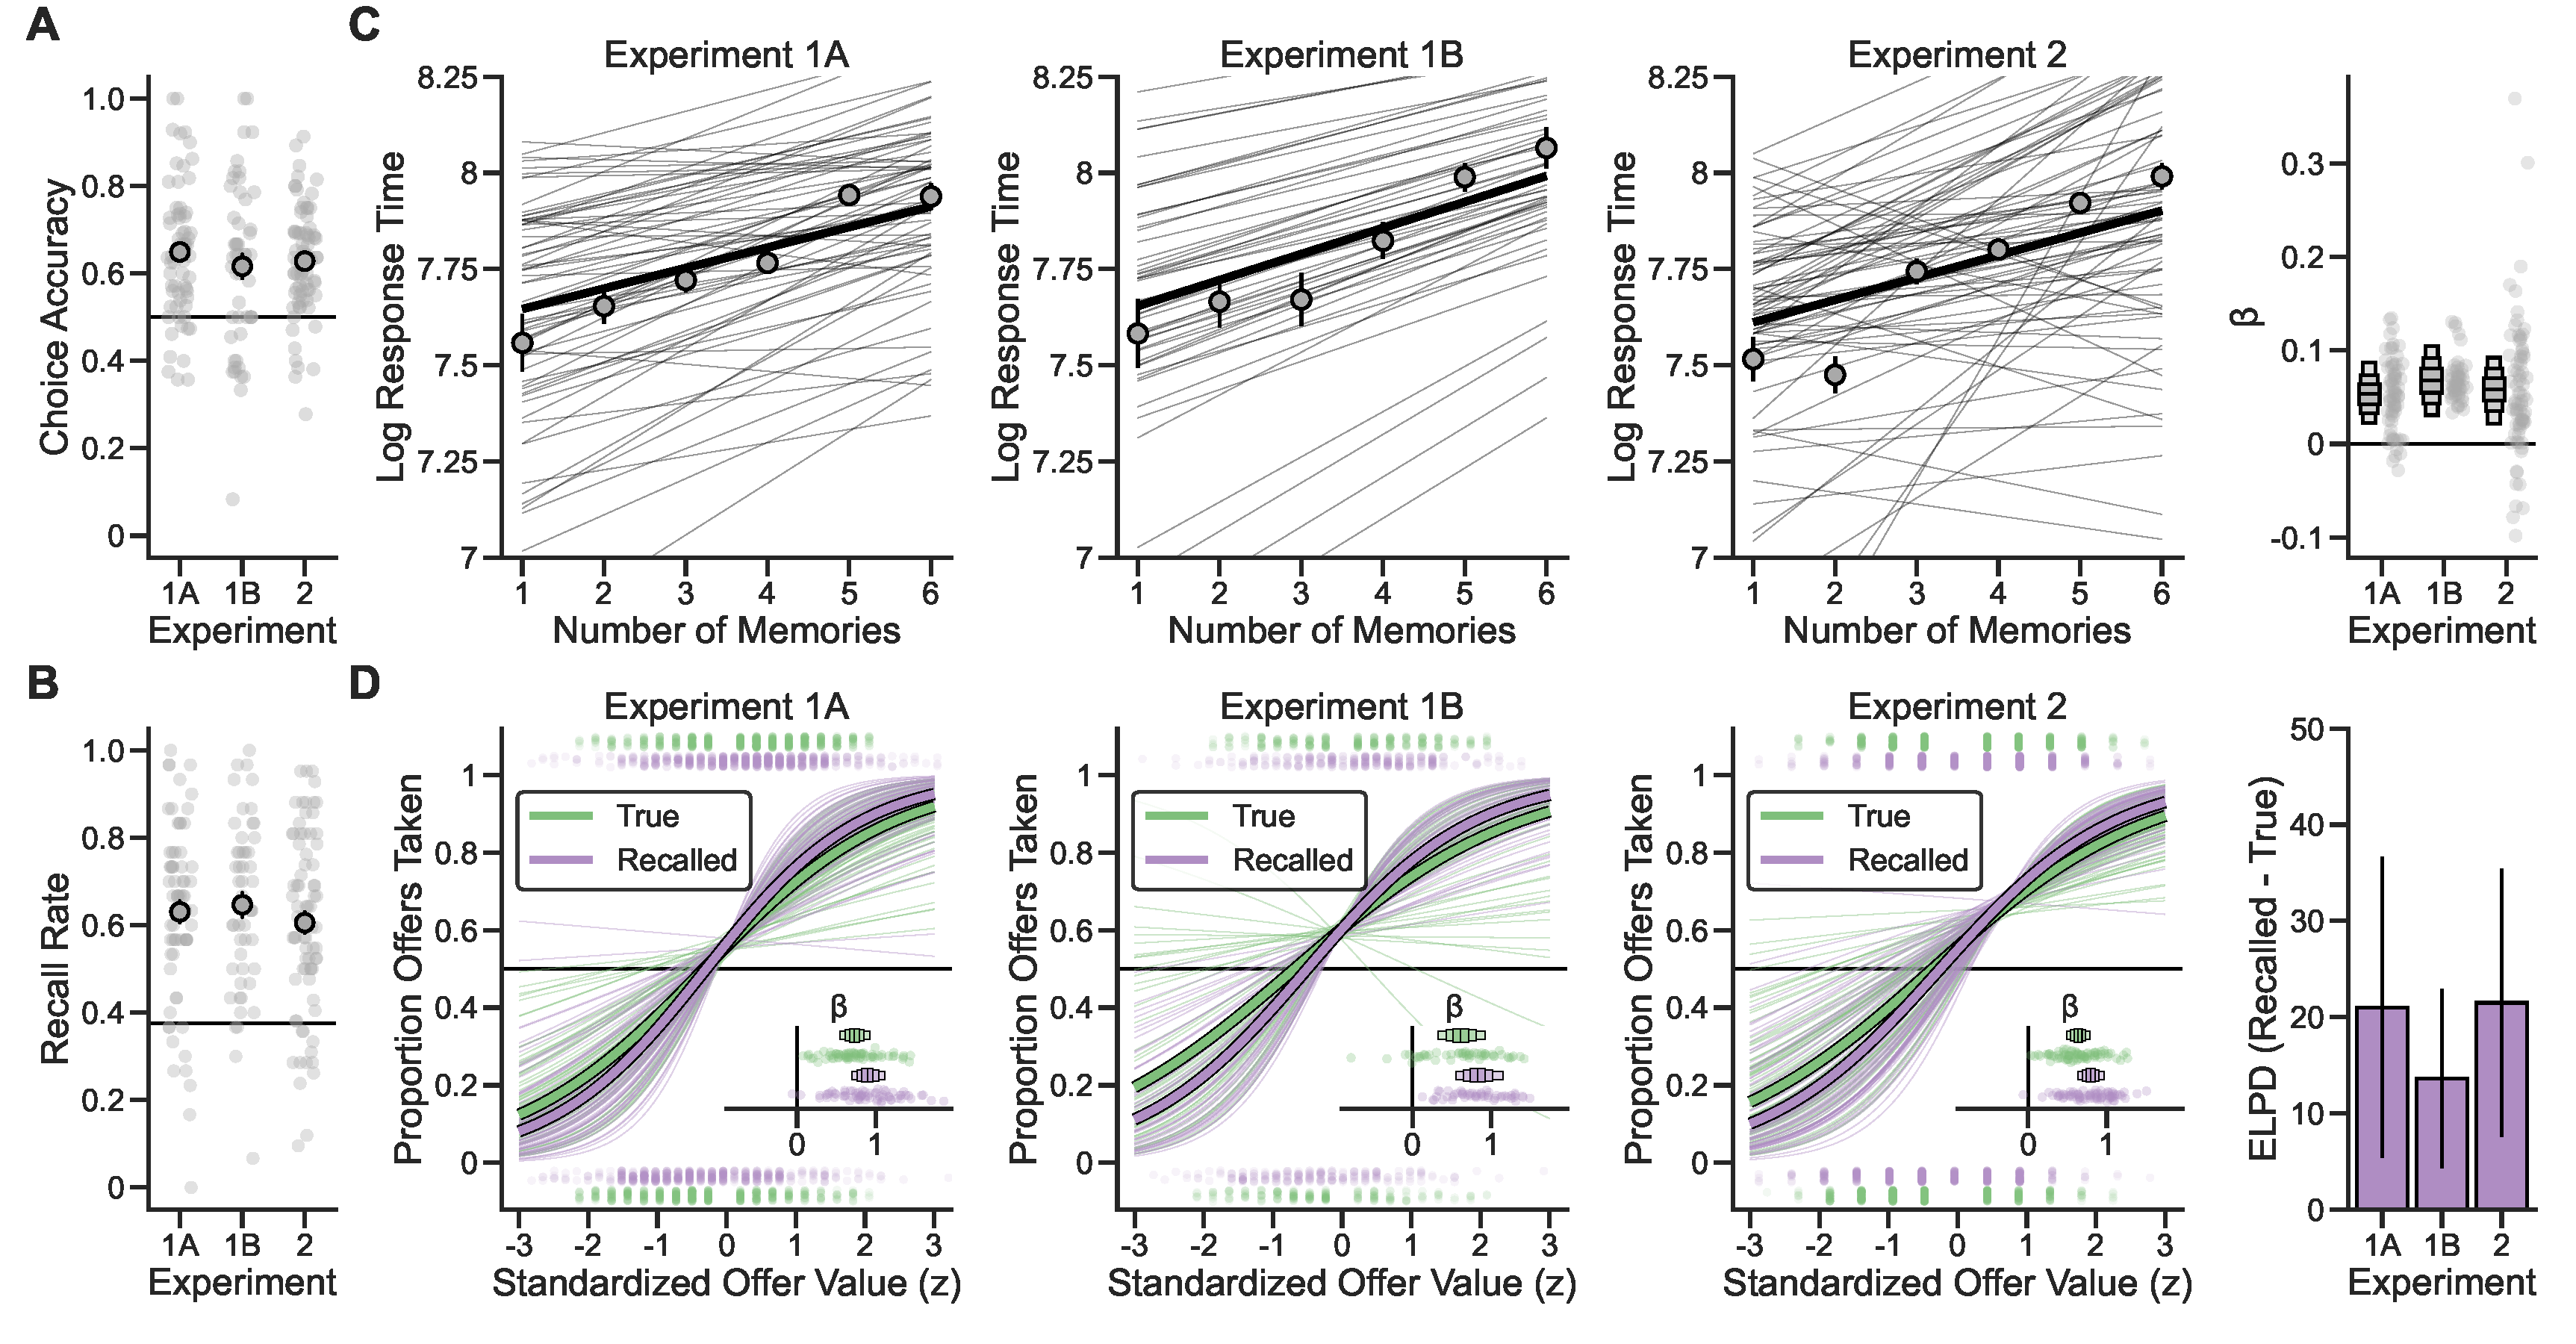
\includegraphics[width=1\textwidth]{figures/Figure2.pdf}
    \caption{People use episodic memory to make decisions in multi-feature environments. \textbf{A)} Participants' overall choice accuracy during the decision phase, shown for Experiment 1 (Samples A and B) and Experiment 2. Chance performance is represented by the horizontal line. Large points represent-group-level averages with error bars representing standard error. Small points represent average choice accuracy for individual participants. \textbf{B)} Participants' rate of accurately recalling items seen in each round during the free recall portion of the memory phase. Recall rates were defined as the proportion of items that were accurately recalled relative to all items that were shown. Chance performance is represented by the horizontal line. Large points represent group-level averages with error bars representing standard error. Small points represent average recall rates for individual participants. \textbf{C)} Participants' decision response times (log transformed) as a function of the number of memories that they accurately recalled on each round. Large lines represent group-level fits of a mixed-effects linear regression model, with individual fits plotted as smaller lines. Points represent group-level averages with uncertainty represented as standard error. Far right panel: Fixed effects and random effects slopes (beta) for regression model fits. Boxes represent the fixed effects posterior distribution, with horizontal lines representing the mean and boxes representing 50\%, 80\%, and 95\% HDIs. Points represented the random effect slopes for each subject. \textbf{D)} Left: The proportion of offers that were taken as a function of summed true offer value and recalled offer value. Offer values are z-scored to facilitate comparison. Inlays show the mixed effects slopes for each predictor. Far right panel: Results of comparing the true and recalled offer value models. Model fit was first assessed using 10-fold cross-validation. The expected log pointwise predictive density (ELPD) was then computed. Higher ELPD values indicate a higher likelihood of accurately predicting new data. Here the difference in ELPD between models is shown such that positive values provide more support for the recalled offer value model. Uncertainty in the comparison is shown as the standard error of this difference, calculated as in Vehtari et al. (2017)\cite{vehtariPracticalBayesianModel2017}.}
    \label{fig:figure2}
\end{figure*}

\section{Results}

\subsection{Episodic memory allows access to details from past events for decision making}

In experiment one, we first aimed to test whether people primarily rely on episodic memory rather than feature-based selective attention when making decisions in environments with multiple features. We hypothesized that the computational demands of tracking multiple features simultaneously would make a feature-based strategy impractical, leading participants to instead use episodic memory to compute offer values at the time of choice. We tested this hypothesis in two independent samples to ensure the replicability of our findings. Before addressing our primary question, we first examined whether participants learned to make effective decisions in the task. At the group-level, participants in both samples tended to take positive and to leave negative offers (Sample A: $M_{accuracy} = 63.6\% \pm 1.5$, $\beta_{0} = 0.46, 95\% \ HDI = [0.33, 0.59]$; Sample B: $M_{accuracy} = 60.8\% \pm 2.3$, $\beta_{0} = 0.36, 95\% \ HDI = [0.17, 0.55]$), despite substantial inter-individual variability (\textbf{Figure 2A}). Participants' choices therefore reflected their ability to compute the value of each offer by summing over individual experiences.

Our next goal was to examine whether participants maintained memory traces for the individual episodes they encoded in the first part of each round. To accomplish this, our experiment required participants to complete an additional memory phase immediately after the decision making phase of each round (\textbf{Figure 1A}). This memory phase consisted of two parts in which participants were asked to remember both elements of the episodes they had seen: they were first asked to freely recall each of the six items from a round, and then to recall the reward that was associated with each item. Participants had robust memory for the individual episodes, remembering between three and four items, on average (Sample A: $M_{recall} = 63\% \pm 2.5$; Sample B: $M_{recall} = 64.7\% \pm 2.8$; \textbf{Figure 2B}), which was well above chance-level recall (Sample A: $\beta_{0} = 0.26, 95\% \ HDI = [0.20, 0.31]$; Sample B: $\beta_{0} = 0.27, 95\% \ HDI = [0.22, 0.33]$). Item recalls exhibited classic properties of episodic memory, with items presented close together during encoding being more likely to be recalled consecutively (temporal contiguity effect\cite{kahanaFoundationsHumanMemory2012}; \textbf{Figure S2}), providing further evidence that participants engaged episodic memory during the task. Participants also accurately remembered the rewards associated with each item, showing a strong positive relationship between remembered and actual rewards (Sample A: $\beta_{reward} = 0.52, 95\% \ HDI = [0.44, 0.59]$; Sample B: $\beta_{reward} = 0.47, 95\% \ HDI = [0.37, 0.56]$; \textbf{Figure S3}). These results demonstrate that participants formed and retained strong memories for each episode beyond the decision making phase, and that individual memories were available for potential recall at choice time.

Next, in order to disambiguate between the episodic and feature-based strategies, we used participants' responses on the memory phase to analyze their choice behavior. First, we reasoned that recalling an individual episode should take time\cite{ratcliffTheoryMemoryRetrieval1978, sederbergContextbasedTheoryRecency2008, kahanaFoundationsHumanMemory2012} and that, accordingly, the amount of time it takes to make a decision should scale with the number of episodes that are referenced (\textbf{Figure 1C}). Importantly, the feature-based strategy makes no such prediction, as only a single item (a precomputed offer value) must be retrieved at choice time. To test this idea, we first used participants' free recall data to determine the total number of items that they accurately recalled on each round of the task. We then examined whether they took longer to respond to offers during rounds on which they recalled more items overall. As predicted, participants took longer to decide when they subsequently recalled more memories (Sample A: $\beta_{nMemories} = 0.05, 95\% \ HDI = [0.02, 0.08]$; Sample B: $\beta_{nMemories} = 0.07, 95\% \ HDI = [0.03, 0.11]$; \textbf{Figure 2C}). We next conducted a complementary analysis examining whether decision response times were specifically related to the number of offer-relevant memories recalled --- that is, only those memories whose features matched each offer (e.g., only recalled red items for offers about red things). Interestingly, we found no consistent relationship between response times and the number of offer-relevant memories recalled (see \textbf{Table S1} for results across all experiments). Together, these results suggest that rather than accessing only the memories that are strictly needed for each decision, participants retrieved all of their available memories, presumably selecting from these memories only the trial-relevant information before making a choice.

Having established that participants appeared to access individual memories during their decisions, we moved to examine the actual choices they made. We reasoned that if their decisions were based on the rewards they remembered being associated with each item, as predicted by an episodic strategy, their choices should be sensitive to the summed value of these remembered rewards (\textbf{Figure 1C}). To test this, we used participants' responses on the reward memory portion of the memory phase to determine the \textit{recalled value} of each offer. Specifically, we summed over the reported remembered reward of each offer-relevant item that was also recalled during the free recall phase. In contrast, we expected that evidence for a feature-based strategy would manifest as choices being primarily driven by the \textit{true value} of each offer, independent of what participants explicitly remembered. This prediction follows from the nature of feature-based learning: if participants precomputed feature values during encoding, these cached values would be immune to later forgetting or distortions of individual episodes. To arbitrate between these possibilities, we fit two logistic regression models to participants' choices: one that used the true offer value to predict each choice, and another that used recalled offer value to predict each choice. We then compared the out-of-sample predictive accuracy of each model using cross-validation.

While participants' choices were sensitive to both true offer value (Sample A: $\beta_{true} = 0.73, 95\% \ HDI = [0.56, 0.91]$; Sample B: $\beta_{true} = 0.61, 95\% \ HDI = [0.32, 0.92]$) and recalled offer value (Sample A: $\beta_{recalled} = 0.89, 95\% \ HDI = [0.69, 1.11]$; Sample B: $\beta_{recalled} = 0.83, 95\% \ HDI = [0.55, 1.15]$), recalled offer value was slightly more effective at predicting held-out choices in both samples (Sample A: $ELPD_{recalled-true} = 21.00 \pm 15.63$, Sample B: $ELPD_{recalled-true} = 13.58 \pm 9.30$; \textbf{Figure 2D}, \textbf{Table S2}). This result indicates that participants tended to rely more heavily on the information contained in individual episodes, namely the identity and value of items, to make their decisions.

One limitation of this experiment is that it does not distinguish between two fundamentally different ways that information could be represented in memory. One possibility, which we have suggested so far, is that experiences are stored as integrated episodes, where multiple features are bound together into a single conjunctive representation (e.g., "butterfly")\cite{oreillyHippocampalConjunctiveEncoding1994, oreillyConjunctiveRepresentationsLearning}. Alternatively, individual experiences could be stored as separate features (e.g., "blue" and "animal" as independent elements)\cite{rudyConjunctiveRepresentationsHippocampus2001}. Although both approaches could support value computation in our task, the latter becomes increasingly challenging as more features must be maintained and retrieved. To test this idea, we conducted a second experiment that was nearly identical to experiment one, but where we doubled the number of features associated with each stimulus (\textbf{Figure S1}). We reasoned that if participants relied upon memories comprised of separate features, this increased complexity would impair performance. Conversely, if participants encoded integrated episodes, the natural binding of features should preserve performance despite the additional complexity. As predicted, performance on experiment two was comparable to experiment one and all results replicated (\textbf{Figure 2}, \textbf{Table S3}), supporting the conclusion that participants relied on integrated episodic memories rather than separate feature memories to complete the task.

Together, these results demonstrate that when faced with choices that could be based on many different features, participants primarily employed an episodic strategy that involved retrieving and computing over individual memories at choice time. This finding suggests that despite the increased computational demands during decision making, people prefer to maintain detailed episodic memories that can be flexibly accessed rather than attempting to track and update values for multiple features simultaneously. This preference may reflect the difficulty of implementing a feature-based strategy when faced with the curse of dimensionality, as suggested by previous theoretical work\cite{gershmanReinforcementLearningEpisodic2017}.

\subsection{Episodic memory enables flexible decision making when it is unclear which details are important}

Our findings so far demonstrate that people rely on episodic memory to make decisions in multi-feature environments, in part because episodic memories provide a natural solution to the curse of dimensionality. However, this observation alone does not fully explain why episodic memory might be specifically advantageous for decision making. To address this, we next hypothesized that episodic memory's key benefit lies in its ability to enable flexible decisions when future task demands are uncertain --- a common situation in the real world. This hypothesis predicts that people should shift away from using episodic memory when they can anticipate which features will be relevant for their upcoming decisions, as this foreknowledge would make a feature-based strategy more viable. To test this prediction directly, we next conducted an experiment where we manipulated whether participants knew in advance which features would be relevant for their decisions.

In experiment three, we contrasted two conditions: one where participants learned which features would be relevant only at choice time (\textit{after} encoding), and another where participants knew \textit{before} encoding which features would be needed for their upcoming decisions (\textbf{Figure 1C}). Specifically, in this new before condition, participants were told prior to encoding that they would later receive offers about color or category, but not both. This manipulation created conditions where the feature-based strategy is more feasible, as participants could safely ignore irrelevant features (e.g., category when only color offers would be made). This advantage was absent in the after condition, where feature relevance remained uncertain during encoding. We predicted that people would primarily rely on an episodic strategy in the after condition, but would shift toward a feature-based strategy when feature relevance was known in advance. We again tested this prediction across two independent samples to ensure the replicability of our findings.

% Figure 3
\begin{figure*}[t]
    \centering
    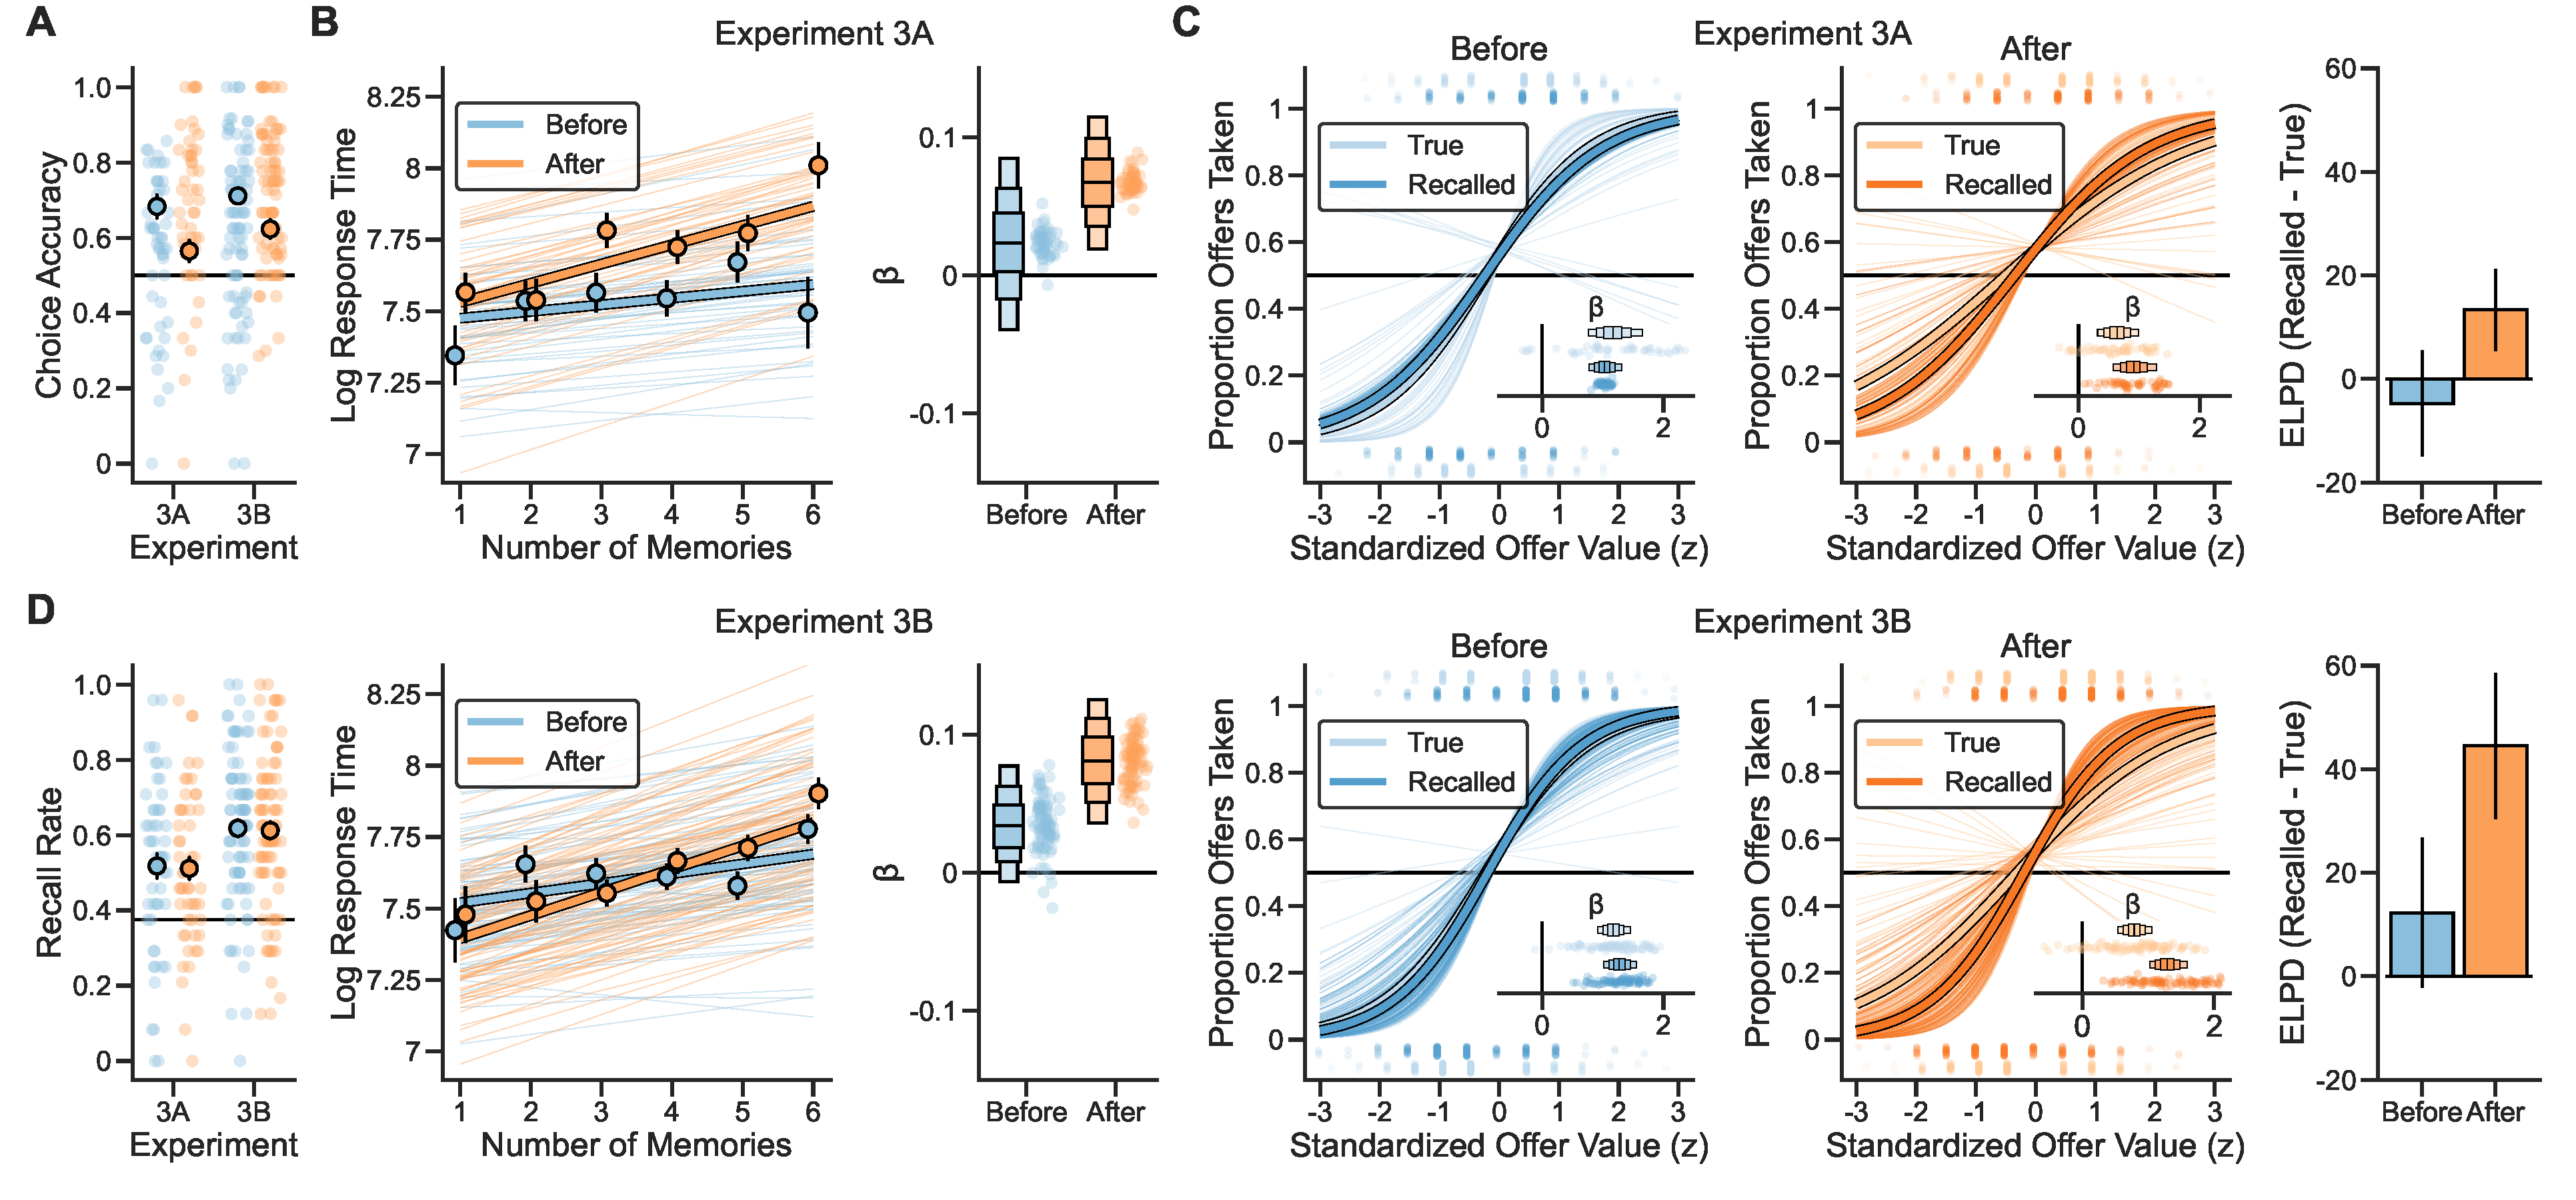
\includegraphics[width=1\textwidth]{figures/Figure3.pdf}
    \caption{Episodic memory is primarily used for decisions when it is unclear what features are important. \textbf{A)} Participants' choice accuracy during the decision phase, shown for Experiment 3 (samples A and B). Decisions made when the future relevance of features was known at encoding (the before condition, in blue) are shown separately from those made when this information was unknown at encoding (the after condition, in orange). Large points represent-group-level averages with error bars representing standard error. Small points represent average choice accuracy for individual participants. \textbf{B)} Participants' decision response times (log transformed) as a function of the number of memories they accurately recalled on each round for sample A (top) and sample B (bottom). Left: Large lines represent the group-level fit of a mixed-effects regression, with individual subject fits plotted as smaller lines. Points represent group-level averages with standard error. Right: Fixed effect slopes and random effect slopes (beta) for regression model fits. Boxes represent the fixed effects posterior distribution, with horizontal lines representing the mean and boxes representing 50\%, 80\%, and 95\% HDIs. Points represent random effect slopes for each subject. \textbf{C)} The relationship between choices and offer value for sample A (top) and sample B (bottom). Left: The proportion of offers taken as a function of summed true offer value and recalled offer value for the Before and After conditions. Mixed effects slopes are plotted as inlays. Right: Model comparison showing the difference in ELPD alongside standard error. \textbf{D)} Participants' rate of accurately recalling items seen in each round during the free recall portion of the memory phase. Chance performance is represented by the horizontal line. Large points represent group-level averages with error bars representing standard error. Small points represent average recall rates for individual participants.}
    \label{fig:figure3}
\end{figure*}

Participants responded accurately, primarily taking positive and leaving negative offers both during rounds in which feature relevance was communicated before encoding (Sample A: $M = 68.5\% \pm 2.9$, $\beta_{0} = 0.86, 95\% \ HDI = [0.62, 1.33]$; Sample B: $M = 71.7\% \pm 1.9$, $\beta_{0} = 1.00, 95\% \ HDI = [0.81, 1.21]$) and after encoding (Sample A: $M = 59.7\% \pm 2.9$, $\beta_{0} = 0.43, 95\% \ HDI = [0.20, 0.66]$; Sample B: $M = 63.3\% \pm 2.2$, $\beta_{0} = 0.62, 95\% \ HDI = [0.41, 0.83]$; \textbf{Figure 3A}). Notably, participants chose more accurately in the before condition (by an average of 8.8\% and 8.4\% in each sample, respectively), suggesting that there were clear benefits to performance when feature relevance was known during encoding. Importantly, though, performance in the after condition was on par with our prior experiments.  

We next aimed to test our primary hypothesis. As predicted, in the after condition participants took longer to make decisions when they recalled more memories (Sample A: $\beta_{nMemories} = 0.08, 95\% \ HDI = [0.04, 0.12]$; Sample B: $\beta_{nMemories} = 0.06, 95\% \ HDI = [0.02, 0.11]$; \textbf{Figure 3B}). Yet, we found little evidence for this relationship in the before condition, when participants were aware of which features they would need for their future decisions (Sample A: $\beta_{nMemories} = 0.02, 95\% \ HDI = [-0.04, 0.07]$; Sample B: $\beta_{nMemories} = 0.03, 95\% \ HDI = [-0.01, 0.07]$). We then further examined the extent to which true and recalled offer value predicted participants' choices in both conditions. We expected recalled offer value to be a better predictor of choices in the after condition, but not in the before condition, if participants retrieved episodes during decisions made in the former but not the latter. In line with this prediction, recalled offer value better predicted held-out choices in the after condition but not in the before condition in both samples (\textbf{Figure 3C}, \textbf{Table 1}; see \textbf{Table S2} for performance of all models). These results indicate that participants primarily referenced individual episodes during decision making when it was unclear at encoding which features would be needed for future decisions.

To better understand the source of these differences in strategy recruitment, we next examined participants' performance on the memory phase. Specifically, while participants shifted away from using episodic memory when feature relevance was known prior to decision making, it is unclear whether this effect emerged from changes in how experiences were initially encoded or from whether they were later accessed during decision making. We reasoned that if participants strategically modified their encoding based on known feature relevance, they should show impaired subsequent memory for individual episodes in the before condition, as they would be focused primarily on computing and maintaining feature-level values rather than encoding complete episodic memories. However, another possibility is that participants instead continued to encode episodic memories alongside precomputing feature values, consistent with evidence that these distinct systems often operate in parallel during learning\cite{nicholasUncertaintyAltersBalance2022a, bornsteinRemindersChoicesBias2017a, leeNeuralComputationsMediating2015, packardInactivationHippocampusCaudate1996, poldrackCompetitionMultipleMemory2003}. In this case, we expected to see comparable memory performance between conditions, with task demands influencing whether these memories were later accessed at choice time rather than whether they were initially stored.

Across both samples, we found that participants maintained strong memories of the episodes encountered in each round regardless of condition. Participants accurately recalled individual items with no differences in recall rates between conditions (Sample A: $\beta_{after-before} = -0.01, 95\% \ HDI = [-0.10, 0.08]$; Sample B: $\beta_{after-before} = -0.01, 95\% \ HDI = [-0.07, 0.06]$; \textbf{Figure 3D}; \textbf{Table 2}), and they further showed equally similar memory for the rewards associated with each item (Sample A: $\beta_{after-before} = -0.06, 95\% \ HDI = [-0.18, 0.06]$; Sample B: $\beta_{after-before} = -0.05, 95\% \ HDI = [-0.15, 0.05]$; \textbf{Figure S3}; \textbf{Table 2}). These findings demonstrate that participants encoded complete episodic memories regardless of whether they knew which features would be relevant for future decisions.

Together, these results provide evidence that people selectively use episodic memory for decision making when feature relevance is unknown during encoding. When participants were aware of which features would be important for decision making prior to encoding, our results suggested that they no longer retrieved individual memories at choice time. This shift toward the feature-based strategy is sensible --- it reduces computational demands at decision time by allowing direct access to pre-computed feature values rather than requiring the retrieval and integration of multiple episodic memories. This approach led to improved performance on expected decisions because the episodic strategy can introduce noise (e.g. though errors in memory retrieval), especially under time constraints when only a subset of memories might be accessible. Yet we also found that participants maintained detailed episodic memories in both conditions, suggesting that the differences we observed during decision making emerged from how information was accessed at choice time rather than how it was initially encoded. We next aimed to determine whether this parallel maintenance of episodic memories provided its own adaptive benefits for decision making.

\begin{table*}[t]
\centering
\begin{tabular}{llccc}
\hline
Condition & Sample & Model & $\beta$ [95\% HDI] & ELPD$_{Recalled-True}$ ± SE \\
\hline
Before & A & True & 1.17 [0.76, 1.65] & -4.74 ± 10.22 \\
       &   & Recalled & 1.02 [0.77, 1.31] & \\
       & B & True & 1.17 [0.92, 1.46] & 12.26 ± 14.50 \\
       &   & Recalled & 1.27 [1.02, 1.55] & \\
\hline
After  & A & True & 0.63 [0.31, 0.99] & 13.32 ± 7.96 \\
       &   & Recalled & 0.91 [0.58, 1.28] & \\
       & B & True & 0.79 [0.54, 1.06] & 44.50 ± 14.13 \\
       &   & Recalled & 1.29 [1.03, 1.59] & \\
\hline
\end{tabular}
\caption{Experiment 3 model comparison results showing fixed effects estimates ($\beta$) with 95\% highest density intervals (HDI) and difference in expected log pointwise predictive density (ELPD) between true and recalled offer value models.}
\label{tab:modelcomparison}
\end{table*}

\begin{table*}[t]
\centering
\begin{tabular}{llcccc}
\hline
Experiment & Sample & Condition & Recall Rate ± SE & $\beta_0$ [95\% HDI] & $\beta_{reward}$ [95\% HDI] \\
\hline
3 & A & Before & 51.8\% ± 3.2 & 0.14 [0.08, 0.21] & 0.55 [0.48, 0.62] \\
  &   & After & 51.1\% ± 2.9 & 0.14 [0.08, 0.19] & 0.49 [0.39, 0.57] \\
  & B & Before & 61.8\% ± 2.2 & 0.24 [0.20, 0.29] & 0.53 [0.46, 0.60] \\
  &   & After & 61.2\% ± 2.3 & 0.24 [0.19, 0.28] & 0.48 [0.41, 0.55] \\
4 & - & Before & 62.5\% ± 1.9 & 0.25 [0.21, 0.29] & 0.54 [0.49, 0.59] \\
  &   & After & 61.9\% ± 1.9 & 0.23 [0.19, 0.27] & 0.48 [0.42, 0.54] \\
\hline
\end{tabular}
\caption{Memory performance across experiments 3 and 4. Recall Rate shows mean percentage of items recalled (± standard error). $\beta_0$ represents the intercept of a model predicting recall performance relative to chance. $\beta_{reward}$ represents the slope of a model predicting the relationship between remembered and actual rewards.}
\label{tab:memory}
\end{table*}

\subsection{Episodic memory maintains access to details if they become unexpectedly relevant}

The results of experiment three suggest that while participants appeared to rely on a feature-based strategy when feature relevance was known in advance, they still maintained detailed episodic memories. One prediction that follows from this observation is that participants should still be able to use their episodic memories to maintain access to features they had initially deemed irrelevant in order to inform their decisions. In contrast, if participants abandoned episodic encoding entirely, they should struggle to access information about these irrelevant features.

We designed a fourth experiment in order to test this idea. In experiment four, once participants had completed eight rounds where the manipulation introduced by experiment three was honored, we asked them to complete a final additional round in which they were shown all possible offers. Importantly, participants were shown these \textit{unexpected} offers regardless of whether they had been told before the encoding phase of this final round that they would see only a subset of offers later on. This allowed us to examine performance when the final round was completed under the before condition for both expected and unexpected offers. By definition, all offers shown during the after condition were unexpected. We additionally modified the task to create conditions that would encourage greater reliance on the feature-based strategy. To accomplish this, we simplified the decision phase by presenting only a single offer type per round (e.g., "red") prior to the final round. This modification meant that participants in the before condition needed to track only one specific feature value rather than multiple instances of the same feature (e.g., just "red" instead of all colors), making the feature-based strategy exceptionally efficient. We predicted that this change would lead participants to rely more heavily on the feature-based strategy in the before condition relative to experiment three.

We further predicted that participants should show a specific pattern of choice behavior if they maintained access to their episodic memories despite this increased commitment to the feature-based strategy. First, in response to unexpected final round offers completed under the before condition, we predicted that participants' accuracy should drop relative to their performance on previous rounds. This is because they would no longer be able to rely on the feature-based strategy, which provided clear benefits to performance (improving accuracy by 8-9\% in experiment three when feature relevance was known in advance). Second, we predicted that to make these unexpected decisions, participants would instead need to fall back on using their episodic memories, leading to accuracy levels similar to their performance in the after condition.

% Figure 4
\begin{figure*}[t]
    \centering
    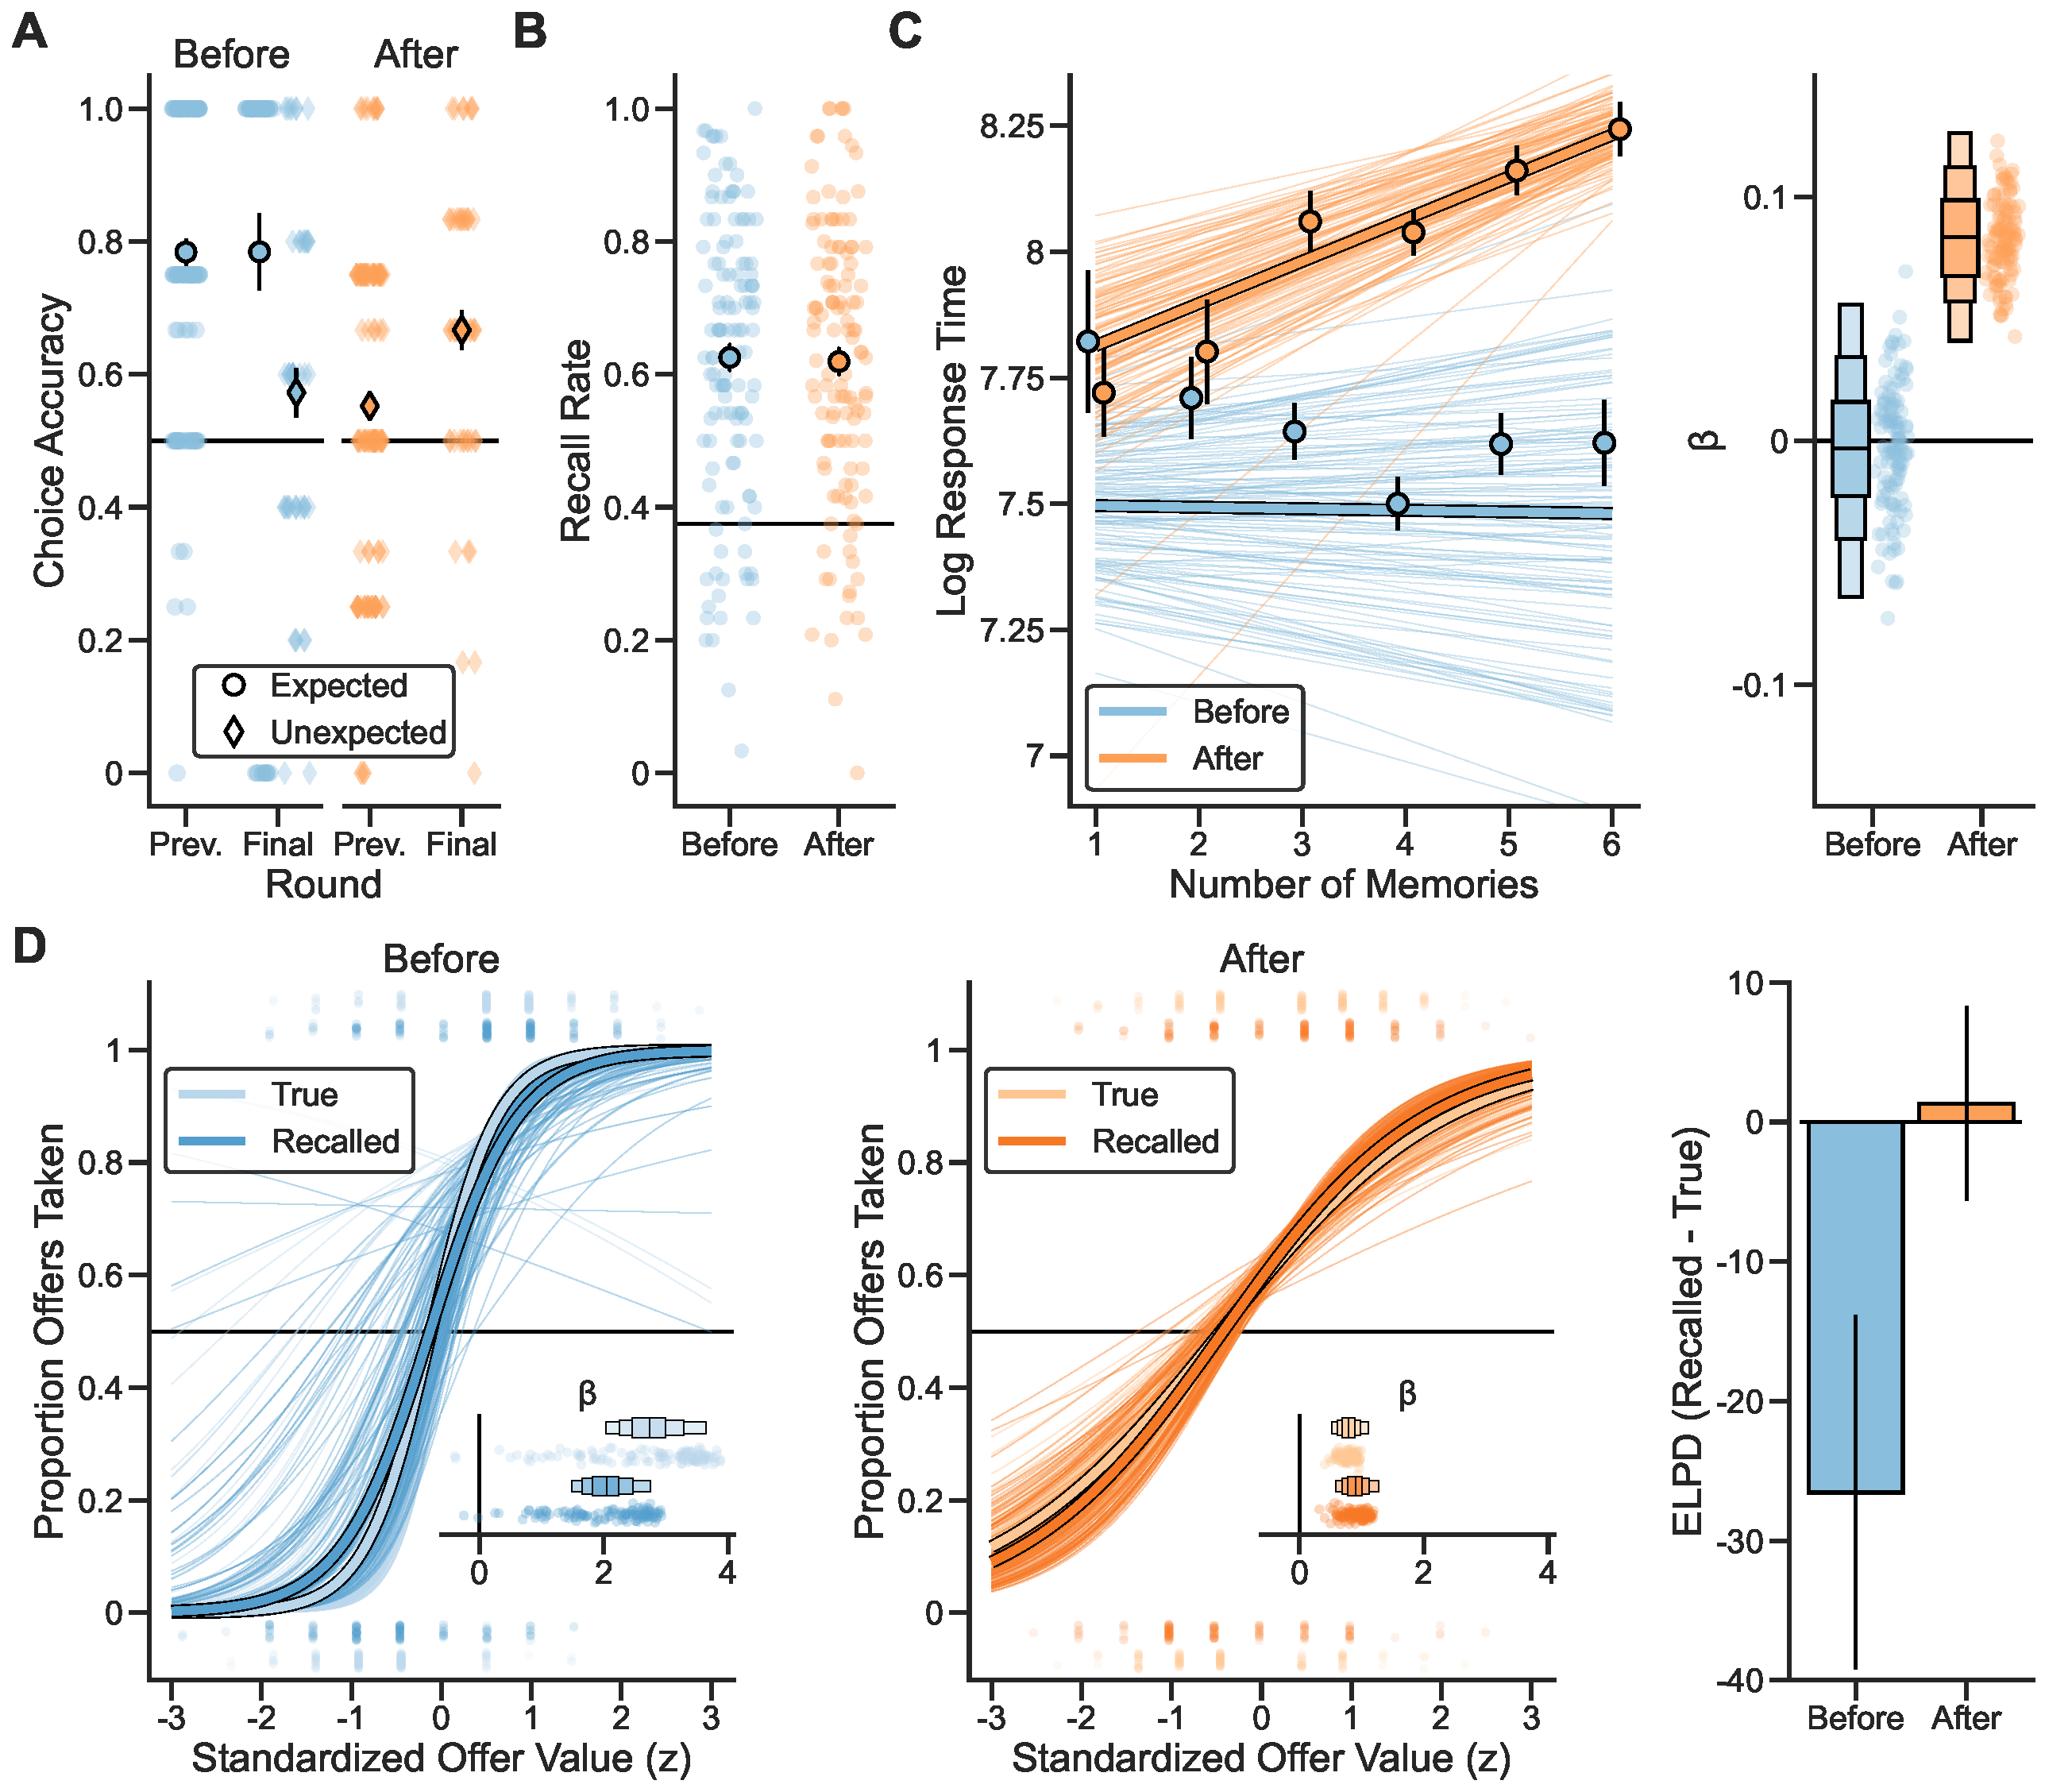
\includegraphics[width=0.7\textwidth]{figures/Figure4.pdf}
    \caption{Episodic memory is used to make choices about unexpected offers. \textbf{A)} Experiment 4 choice accuracy, separated by all rounds prior to the final round (labeled as previous rounds) and the final round in which participants were asked to make decisions about both offers they expected (in the before condition) as well as those that were unexpected (in both conditions). Large points represent-group-level averages with error bars representing standard error. Small points represent average choice accuracy for individual participants. By design, only a single offer was expected in the before condition. \textbf{B)} Participants' rate of accurately recalling items seen in each round of experiment 4 during the free recall portion of the memory phase. Chance performance is represented by the horizontal line. Large points represent group-level averages with error bars representing standard error. Small points represent average recall rates for individual participants. \textbf{C)} Experiment 4 participants' decision response times (log transformed) as a function of the number of memories they accurately recalled on each round. Left: Large lines represent the group-level fit of a mixed-effects regression, with individual subject fits plotted as smaller lines. Points represent group-level averages with standard error. Right: Fixed effect slopes and random effect slopes for regression model fits. Boxes represent the 
    fixed effects posterior distribution, with horizontal lines representing the mean and boxes representing 50\%, 80\%, and 95\% HDIs. Points represent random effect slopes for each subject. \textbf{D)} Left: The proportion of offers taken as a function of summed true offer value and recalled offer value for the before and after conditions. Mixed effects slopes are plotted as inlays. Right: Model comparison showing the difference in ELPD alongside standard error.}
    \label{fig:figure4}
\end{figure*}

We first examined overall performance on rounds prior to the final round, finding that while participants responded accurately in both conditions (Before: $M = 78.4\% \pm 2.0$, $\beta_{0} = 1.57, 95\% \ HDI = [1.29, 1.90]$; After: $M = 55.2\% \pm 2.2$, $\beta_{0} = 0.52, 95\% \ HDI = [0.32, 0.74]$; \textbf{Figure 4A}), they performed substantially better in the before condition relative to both samples in experiment three. Participants further showed equivalent memory performance across both conditions, with no differences in recall rates ($\beta_{after-before} = -0.02, 95\% \ HDI = [-0.07, 0.04]$; \textbf{Figure 4B}; \textbf{Table 2}) or in memory for associated rewards ($\beta_{after-before} = -0.06, 95\% \ HDI = [-0.14, 0.02]$; \textbf{Figure S3}; \textbf{Table 2}). These results suggest that although participants were more capable at deciding in the before condition when they had to compute only the value of a single feature, they still separately maintained episodic memories.

We next asked whether this increase in performance in the before condition was due to participants' greater reliance on the feature-based strategy. In line with this interpretation, we found that during the before condition there was virtually no evidence of a positive relationship between the number of memories recalled and decision response times ($\beta_{nMemories} = -0.02, 95\% \ HDI = [-0.07, 0.02]$; \textbf{Figure 4C}), and participants' choices were better predicted by true offer value ($\beta_{true} = 2.74, 95\% \ HDI = [2.03, 3.65]$) than recalled offer value ($\beta_{recalled} = 2.04, 95\% \ HDI = [1.49, 2.75]$, $ELPD_{recalled-true} = -26.54 \pm 12.69$; \textbf{Figure 4D}, \textbf{Table S2}). In contrast, in the after condition, participants showed longer decision response times when more memories were recalled ($\beta_{nMemories} = 0.09, 95\% \ HDI = [0.05, 0.12]$). While participants' choices in this condition were numerically more sensitive to recalled offer value ($\beta_{recalled} = 0.90, 95\% \ HDI = [0.59, 1.27]$) than true offer value ($\beta_{true} = 0.79, 95\% \ HDI = [0.52, 1.10]$), both models were equally capable of predicting held-out choices ($ELPD_{recalled-true} = 1.33 \pm 6.97$; \textbf{Figure 4D}). This equivalent model performance likely reflects the limited data available for cross-validation, as participants made substantially fewer decisions per condition in this experiment compared to experiment three.

Finally, we turned to test the primary question of this experiment: whether in the final round participants maintained access to information about the features they were told would be irrelevant for future decisions. As predicted, participants who completed their final round in the before condition showed impaired performance on unexpected offers compared to their performance on prior rounds in this condition ($M = 57.3\% \pm 3.7$, $\beta_{0} = 0.14, 95\% \ HDI = [0.04, 0.24]$; \textbf{Figure 4A}), but maintained high accuracy on expected offers ($M = 78.4\% \pm 5.8$, $\beta_{0} = -0.07, 95\% \ HDI = [-0.20, 0.06]$). Critically, participants' performance on unexpected offers matched that of the prior rounds in the after condition ($\beta_{0} = -0.02, 95\% \ HDI = [-0.11, 0.07]$), suggesting they could successfully fall back on episodic memories when the feature-based strategy was insufficient. Surprisingly, we also found that participants who completed their final round in the after condition exceeded their prior performance in this condition ($M = 66.7\% \pm 3.0$, $\beta_{0} = -0.13,  95\% \ HDI = [-0.21, -0.05]$). This improvement may stem from the increased variety of offer types shown in the final round, which provided participants with more opportunities to make decisions about items they successfully remembered, whereas previous rounds with fewer offer types may have tested only items for which their memory was weaker.

The results of experiment four suggest that even under conditions that strongly encouraged reliance on a feature-based strategy, participants maintained detailed episodic memories that they could access when needed. While participants showed clear evidence of using feature-based computations in the before condition, they were still able to rely upon their episodic memories when faced with unexpected offers, performing comparably to the after condition. This pattern of results provides evidence that episodic memory may serve as a "backup" to aid decisions when initially irrelevant features become unexpectedly relevant.

\section{Discussion}

Our findings indicate that people flexibly use episodic memory to guide their choices in multi-feature environments, particularly when future task demands are uncertain. When faced with multiple decision-relevant features (Experiment 1), participants relied primarily on episodic memories to compute offer values during decision making, as evidenced by both their response times and choice patterns. This strategy persisted even as feature complexity increased, suggesting that participants stored experiences as integrated episodes rather than separate feature representations (Experiment 2). When given advance knowledge of feature relevance (Experiment 3), participants shifted toward a more computationally efficient feature-based strategy that involved precomputing values during encoding. Yet despite this shift in strategy, participants continued to encode episodic memories, a parallel operation which proved useful when knowledge about previously irrelevant information was needed for decision making (Experiment 4). Overall, these results demonstrate that episodic memory serves as an adaptive solution to decision making under uncertainty in complex environments, allowing us to flexibly repurpose our memories according to the demands of the present.

This work connects at least two established but largely separate literatures on memory and choice. First, a number of studies focused on decision making have explored the ways in which individual experiences may be recalled for choice\cite{STEWART20061, bieleLearningRiskAttitude2009,plonskyRelianceSmallSamples2015, shadlenDecisionMakingSequential2016, wangMixingMemoryDesire2022}. This research, typically called ``decision by sampling'', proposes that decision variables may be constructed by drawing samples from memory, and explains a number of ways in which peoples' choice behavior differs when information is learned from experience rather than instructed descriptions\cite{hertwigDescriptionExperienceGap2009}. Second, other work has proposed that episodic memory plays a critical role in our ability to infer new information about the world by allowing the formation of new links between past experiences\cite{schlichtingHippocampusMemoryIntegration2017,whittingtonTolmanEichenbaumMachineUnifying2020,bidermanWhatAreMemories2020}. An important but underappreciated part of this role is episodic memory's ability to store multiple features of experience, because each feature provides another opportunity to relate past events with one another. Here we connect these ideas by suggesting that features of episodes may allow for the formation of new decision variables on-the-fly, when they are needed for a choice.

Our findings add to a substantial body of research which has found that the brain contains multiple memory systems that can operate independently yet interact continuously\cite{packardInactivationHippocampusCaudate1996, squireStructureFunctionDeclarative1996, poldrackCompetitionMultipleMemory2003, poldrackInteractiveMemorySystems2001, shohamyHabitsReinforcementLearning2014, montaser-kouhsariTwoRoutesValuebased2024}, with task demands determining which is ultimately recruited for decision making\cite{dawUncertaintybasedCompetitionPrefrontal2005, nicholasUncertaintyAltersBalance2022, leeNeuralComputationsUnderlying2014}. Our results suggest that this parallel operation is adaptive --- while incremental learning can efficiently track relevant statistics when future demands are known, episodic memory may serve as a crucial "backup" system by preserving detailed records of experiences. This is evidenced by participants' ability to successfully encode detailed episodes in experiments three and four even while engaging in the feature-based strategy, and by their ability to use these memories to support unexpected decisions when incremental estimates were poorly calibrated. These findings align with recent computational work\cite{nagyInterplayEpisodicSemantic2025} suggesting that episodic memory may complement incrementally learned summaries by enabling the computation of new task-relevant statistics when unexpected events occur. However, it is important to note that structuring our experiments as a series of rounds --- where participants knew they would be tested on their memory after each decision phase --- may have encouraged them to maintain episodic memories regardless of condition. Future work using a more continuous task design with surprise memory tests is necessary to fully disentangle these possibilities.

Separately, the specific pattern of episodic memory access we observed highlights important limitations of our experimental approach. Specifically, we found that participants' decision times scaled with their total number of memories in each round rather than just those relevant to each offer, suggesting that they retrieved all available memories regardless of their relevance to the current decision. One plausible explanation for this finding is that during their decisions, participants cycled through all of their memories, rejecting those that did not match the current offer. This particular retrieval strategy was enabled by our design --- with only six candidate memories per round and a lengthy response period during each decision --- but it is clearly unrealistic for real-world decisions where we have many more memories to consider. Importantly, extensive research on memory recall suggests that some intrusion of "irrelevant" related memories is inevitable during retrieval\cite{kahanaFoundationsHumanMemory2012}, supporting our general findings even if the specific type of retrieval strategy observed here does not scale. Similarly, our task's simplified feature space, while allowing us to characterize episodic memory use in a controlled setting, still remains far simpler than real world experience, which can consist of vast numbers of features. Although participants' choice behavior was largely unaltered by the addition of new features in experiment two, this setting was still far from naturalistic, and it remains possible that further increases to feature dimensionality could reveal more subtle differences. Moreover, in our design we made the simplifying assumption that episodes consist of perfect recollections of experienced details, when in reality these details are often substantially compressed and abstracted\cite{carmichaelExperimentalStudyEffect1932, nagySemanticCompressionEpisodic2018, zhouPatternSeparationUsing, kerrenExploringRoleDimensionality2025}. Future work using larger memory sets and higher-dimensional stimuli will be important for resolving these issues.

An important next step further lies in characterizing \textit{how} the various organizational principles of episodic memory guide choice. Classic computational models of memory retrieval have formalized how memories are naturally organized and accessed according to their temporal proximity and semantic relationships\cite{howardDistributedRepresentationTemporal2002, polynContextMaintenanceRetrieval2009, kahanaComputationalModelsMemory2020}. This work suggests that when we retrieve a memory, it automatically triggers the recall of other memories that, for instance, occurred nearby in time or share meaningful features. Indeed, participants in our experiments showed a clear tendency to consecutively recall items that were presented close together during encoding (\textbf{Figure S3}). Such organizational principles are likely central to memory-guided decision making, as evidenced by findings demonstrating that choices are systematically influenced by temporally proximate experiences\cite{bornsteinRemindersChoicesBias2017}, by the context present during both encoding\cite{duncanModulatingUseMultiple2019} and decision making\cite{bornsteinReinstatedEpisodicContext2017,duncanModulatingUseMultiple2019}, and by semantic similarity between experiences\cite{plonskyRelianceSmallSamples2015, akaWhatWhatRemember2021}. While our results show that people can effectively use episodic memories for flexible decision making, they do not reveal the specific mechanisms by which memories are accessed. Our behavioral measures were designed to be predicted by basic properties of episodic memory recall and so remain agnostic toward any particular model or sampling algorithm. Indeed, these findings could theoretically arise from many different memory sampling strategies --- from random sampling (as in our toy process model) to more structured retrieval guided by these organizational principles. Applying formal memory models to value-based choice could provide a more precise account of how memories are actually accessed during decision making, while potentially revealing new principles about how memory organization shapes adaptive behavior. Doing so will require not only experimental paradigms that more closely approximate real-world decision making, where people draw upon vast numbers of feature-rich experiences across extended timescales, but also methodology to measure direct memory access during decision making itself.

Related to this point, a critical feature of our experimental design was that we collected memory measures immediately following participants' choices rather than during decision making. We did not ask participants to directly recall items during their decisions because our aim was to assess the strategy participants relied upon without instructing them to use any strategy in particular, and we reasoned that this approach may bias them toward using their episodic memories for choice. One way to circumvent this limitation would be to record neural activity during the decision phase. For example, past approaches using magnetoencephalography (MEG) have successfully decoded both the recall of individual episodes during standard memory tasks\cite{michelmannSpeedTimecompressedForward2019, wimmerEpisodicMemoryRetrieval2020} and the rapid replay of sequences of memories during decision making\cite{liuExperienceReplayAssociated2021, mcfadyenDifferentialReplayReward2023, wimmerDistinctReplaySignatures2023}. One possible future direction would be to similarly attempt to decode memory access during the decision phase of our task design. In addition to providing direct evidence for the recall of individual memories during choice, taking such an approach may provide multiple insights into the ways in which value is computed from memories, for instance by testing hypotheses about the number, temporal order, and semantic relationships between recalled memories during decision making.

In conclusion, our results demonstrate that episodic memory plays an important role in enabling flexible decision making when future task demands are unknown. By maintaining detailed representations of individual experiences, episodic memory allows us to access details from our past if they become relevant for present decisions. This flexibility comes at the cost of increased computational demands during choice, leading people to adopt more efficient strategies based on precomputing decision variables when possible. Recent work on the timing of memory-based decisions supports this view, showing that people proactively compute value from memory whenever circumstances allow them to anticipate future choice requirements\cite{nicholasProactiveReactiveConstruction2025}. Together, these findings suggest that one reason why we maintain detailed memories of the past is to help us flexibly adapt to an uncertain future.

\section{Methods}

\subsection{Experimental Procedure}

Unless otherwise noted, all procedures were identical across experiments, and differences between experiments are summarized in \textbf{Table 3}. Participants completed a four-part task over the course of a single online session designed to measure whether people access individual episodes to make decisions based on multiple features of past experiences (\textbf{Figure 1A}). Completing all four parts (a \textit{round}) took approximately five minutes, and participants completed five (Experiment 1), seven (Experiment 2), or eight (Experiments 3 and 4) rounds in total.

\begin{table}[h]
\centering
\begin{tabular}{p{3cm}p{2.5cm}p{2.5cm}p{2.5cm}p{2.5cm}}
\hline
 & \textbf{Experiment 1} & \textbf{Experiment 2} & \textbf{Experiment 3} & \textbf{Experiment 4} \\
\hline
\textbf{Number of rounds} & 5 & 7 & 8 & 9 \\
\hline
\textbf{Number of stimulus features} & 2: color and category & 4: pattern, location, animacy, size & 2: color and category & 2: color and category \\
\hline
\textbf{Reward range} & -9 to 9 & -2 to 2 & -2 to 2 & -2 to 2 \\
\hline
\textbf{Decisions per round} & Sample A: 6\newline Sample B: 3 & 4 & Sample A: 3\newline Sample B: 3 & 1 (6 in final round) \\
\hline
\textbf{Feature uncertainty manipulation }& No & No & Yes & Yes \\
\hline
\textbf{Surprise choice manipulation} & No & No & No & Yes \\
\hline
\end{tabular}
\caption{Summary of Experimental Differences}
\label{tab:exp_differences}
\end{table}

\subsubsection{Stimuli}

In all experiments except Experiment 2, stimuli varied across two features: color (red, yellow, blue, or green) and category (animal, object, food, scene). In Experiment 2, stimuli instead varied across four binary features: pattern (with or without a pattern), location (aquatic or not aquatic), animacy (animal or object), and size (larger or smaller than a microwave). In all experiments, a total of sixteen possible items were used, with a subset of six pseudo-randomly sampled to be used in each round. All two-feature items and an example subset (highlighted in red) are shown in \textbf{Figure 1B}. As demonstrated in that figure, the six items used in each round were selected such that there were always three items with a specific instantiation of each feature (e.g. three green items, three animals), two of another type (e.g. two blue items, two objects), and one of another type (e.g. one food, one yellow). Items were further selected to be roughly balanced across all rounds and were shown either 2 or 3 times in total.

\subsubsection{Encoding Phase}

In the first part of a round, participants completed a task designed to allow them to encode individual items and an associated reward (which we refer to throughout as an \textit{episode}). Each item was presented on the screen for 1 second, after which its reward appeared alongside it for another 6 seconds. An item's associated reward was a pseudo-randomly sampled integer (excluding 0) between either -9 and 9 (Experiment 1) or between -2 and 2 (Experiments 2, 3, and 4). In order to create a balance of future offer values in each round, the reward assignment algorithm ensured that i) an equal balance of positive and negative reward was used in each round, ii) no feature dimension (e.g. blue or object) had a summed value of exactly zero, and that iii) at least one feature dimension had a positive summed value and at least one had a negative total value. Immediately after viewing the episode, participants completed an attention check consisting of the item alongside two options, either the associated reward that was just shown or another randomly selected reward. They had 3 seconds to respond. Each episode was viewed only once, for a total of six trials per round.

\subsubsection{Distractor Phase}

Immediately following the encoding task, participants completed a 90 second distractor task to prevent active rehearsal of the episodes. This distractor consisted of a 2-back working memory task in which participants were shown one of several letters in sequence. Participants were asked to identify whether the current letter matched the one presented two steps earlier.

\subsubsection{Decision Phase}

Immediately following the distractor task, participants then made up to six decisions based on the features of each item (6 decisions: Experiment 1 (sample A); 4 decisions: Experiment 2; 3 decisions: Experiments 1 (sample B), 3; 1 decision: Experiment 4). Each decision consisted of an offer in which a single feature (e.g. \textit{animal}) was displayed on the screen, and participants were asked to either take or leave this offer. Participants were informed that the value of each offer consisted of the sum of each episode that was described by the offer (e.g. the value of the \textit{animal} offer would be the sum of the rewards associated with all animals seen during encoding), and that they should take positive offers and leave negative offers. Participants had 7.5 seconds to make each decision.

\subsubsection{Memory Phase}

Finally, immediately after the decision task, we assessed participants' memory for the episodes in two ways. First, participants were asked to freely recall the items that they saw in each round. They were provided with six empty text boxes and were told to enter the items in the order in which they remembered them. Participants were further told to halt their recall and move on to the next task if they could no longer remember any items. Following the free recall portion, participants were shown each item and were asked to provide their memory for the reward that was associated with each item.

\subsubsection{Feature Uncertainty Manipulation: Experiments 3 and 4}

In order to determine whether episodic memory is used preferentially when it is unclear which features should be prioritized during encoding, we manipulated whether information was provided to participants about upcoming choices in experiment 3 and 4. In these experiments, participants were told either \textit{before} the encoding phase (4 rounds) or \textit{after} the distractor phase (4 rounds) that they would be shown offers of only one feature type (either color or category) during the decision phase. The order in which participants were shown each condition was counterbalanced.

\subsubsection{Surprise Choice Manipulation: Experiment 4}

We aimed to further test whether participants had access to features that were made irrelevant by the feature uncertainty manipulation, as we predicted that one hallmark of using episodic memory for decision making would be the availability of all of the features of an event at decision time. To accomplish this, we added a final round to experiment 4 where we surprised participants by telling them that regardless of whether they had been told they would only be given offers about one feature or not, they would now need to make decisions about all possible offers.

\subsubsection{Participants}

All experiments were approved by the New York University Institutional Review Board and all participants provided informed consent prior to their participation. Participants with normal or corrected-to-normal vision were recruited from the New York University subject pool. Compensation was provided in the form of course credit. Participants were excluded if they indicated on a post-task questionnaire that they wrote any information down during the study or if they either failed to answer or provided nonsensical responses to the post-task questions. To incentive honest responses on this questionnaire, participants were told that they would receive compensation regardless of their answers.

For Experiment 1 (sample A), 83 participants were recruited and 16 were excluded, leading to a final sample of 67 participants ($M_{age} = 19.05 \pm 0.15$; 23 males, 42 females, 2 declined to say). For Experiment 1 (sample B), 58 participants were recruited and 8 were excluded, leading to a final sample of 50 participants ($M_{age} = 18.76 \pm 0.2$; 14 males, 36 females). For Experiment 2, 90 participants were recruited and 15 were excluded, leading to a final sample of 75 participants ($M_{age} = 18.89 \pm 0.17$; 17 males, 56 females, 2 declined to say). For Experiment 3 (sample A), 61 participants were recruited and 11 were excluded, leading to a final sample of 50 participants ($M_{age} = 18.93 \pm 0.18$; 13 males, 37 females). For Experiment 3 (sample B), 97 participants were recruited and 13 were excluded, leading to a final sample of 84 participants ($M_{age} = 18.81 \pm 0.14$; 25 males, 58 females, 1 declined to say). For Experiment 4, 139 participants were recruited and 14 were excluded, leading to a final sample of 125 ($M_{age} = 19.14 \pm 0.12$; 42 males, 83 females). We recruited a larger sample for Experiment 4 because each participant could complete only one of the before/after conditions during the final "surprise" round, and we aimed to have roughly comparable numbers for each condition to our prior experiments.

\subsection{Model Simulations}

To illustrate the behaviors that allowed us to distinguish between episodic and feature-based decision strategies, we formalized these approaches in two toy process models. The episodic model makes decisions by randomly sampling individual memories and their associated rewards, while the feature-based model precomputes feature-level values during encoding.

For the episodic model, decisions are made by sequentially sampling individual episodes without replacement. Each retrieved episode consists of both the item and its associated reward, with gaussian noise $\sigma$ added to the remembered reward to model noisy recall. The model takes a fixed amount of time $\phi$ to recall each memory. Memory retrieval continues until either: (1) all memories for the round have been retrieved, (2) a time limit is reached, or (3) the model decides to stop retrieving with probability $p_{stop}$ after each recall. To make a choice, the model sums the recalled rewards of all retrieved items that match the current offer's feature (e.g., all recalled red items for an offer about red things). The model then takes the offer if this decision variable is positive and leaves it if it is negative. Lastly, we also included a fixed non-retrieval time, $\rho$, which is added to the total response time for each decision.

In contrast, the feature-based model precomputes the value of each feature during encoding by summing the rewards associated with all items sharing that feature. During the decision phase, the model simply retrieves the cached value for the offered feature and makes a choice according to a logistic choice rule with inverse temperature $\beta$. This strategy predicts constant decision times based on only on a non-retrieval time $\rho$ since only a single cached value must be referenced on each choice.

The models were simulated on the same task structure used with human participants (\textbf{Figure 1C}). We ran 1000 simulations for each model with the following values of each parameter. For the episodic model these were: non-retrieval time $\rho = 1.5$s, recall time $\phi = 0.5$s, reward recall noise $\sigma = 0.5$, stopping probability $p_{stop} = 0.1$, and a maximum decision time of 7.5s. For the feature-based model these were: non-retrieval time $\rho = 1.5$s and inverse temperature $\beta = 5.0$.

\subsection{Statistical Analysis}

All data was analyzed with regression models estimated using hierarchical Bayesian inference such that group-level priors were used to regularize subject-level estimates unless otherwise specified. Predictors were specified as fixed effects alongside random slopes and intercepts that were allowed to vary across subjects. In experiments 3A, 3B, and 4, parameter estimates for rounds completed in either the Before or After conditions were fit separately. The joint posterior was approximated using No-U-Turn Sampling as implemented in stan\cite{hoffmanNoUTurnSamplerAdaptively2014}. Four chains with 2000 samples (1000 discarded as burn-in) were run for a total of 4000 posterior samples per model. Chain convergence was determined by ensuring that the Gelman-Rubin statistic R was close to 1. Default weakly-informative priors implemented in the brms package were used for each regression model\cite{burknerBrmsPackageBayesian2017}. For all models, fixed effects are reported in the text as the mean of each parameter’s marginal posterior distribution alongside 95\% highest density intervals (HDIs), and are shown in figures as 95\%, 80\%, and 50\% HDIs, which each indicate where that percentage of the posterior density falls. Parameter values outside of these ranges are unlikely given the model, data, and priors.

\subsubsection{Response Time Analysis}

To examine how the number of recalled memories impacted the amount of time it took participants to make their choices, we used a linear mixed-effects model to predict trial-wise response times. Response times were modeled using a shifted lognormal distribution, which accounts for the positive skew typical of response times. We included both random intercepts and slopes for participants to account for individual differences in both baseline response speed and sensitivity to the number of memories recalled. The model can be written as:
\begin{align*}
    RT_{ij} &\sim ShiftedLogNormal(\mu_{ij}, \sigma, \theta) \\
    \mu_{ij} &= \beta_0 + \beta_1nMemories_{ij} \nonumber + u_{0j} + u_{1j}nMemories_{ij}
\end{align*}
where $i$ indexes trials and $j$ indexes participants. The parameters $u_{0j}$ and $u_{1j}$ represent the random intercepts and slopes for each participant, $\sigma$ is the scale parameter, and $\theta$ is the shift parameter of the distribution. The number of memories participants recalled in each round ($nMemories_{ij}$) was included as a continuous predictor. We further conducted a separate analysis of the number of offer-relevant memories that participants recalled in each round, which consisted of an identical model but with this predictor instead.

\subsubsection{Decision Analysis}

To analyze the extent to which decision-relevant variables influence participants choices, we fit two  mixed-effects logistic regression models. Binary choices (1 = offer taken, 0 = offer rejected) were predicted by either an offer's true value or its recalled value. The true value of an offer ($TrueValue_{ij}$) was just the sum of all offer-relevant items that were shown to the participants. In contrast, we computed the recalled offer value ($RecalledValue_{ij}$) as the sum over the reward that was remembered for each offer-relevant item that was also recalled during the free recall phase. These predictors were z-scored prior to model fitting in order to facilitate comparison between them. Each model included random intercepts and slopes to account for individual differences in both baseline offer acceptance rates and value sensitivity. These models can be written as:
\begin{align*}
    Choice_{ij} &\sim Bernoulli(p_{ij}) \\
    logit(p_{ij}) &= \beta_0 + \beta_1TrueValue_{ij} \nonumber + u_{0j} + u_{1j}TrueValue_{ij} \\
    logit(p_{ij}) &= \beta_0 + \beta_1RecalledValue_{ij} \nonumber + u_{0j} + u_{1j}RecalledValue_{ij}
\end{align*}

To determine the extent to which either recalled offer value or true offer value best predicted choices, we compared models fit using either predictor. Specifically, model fit was assessed by separating the data into 10-folds and cross validating. The expected log pointwise predictive density (ELPD) was then computed by summing the log likelihood for each held out datapoint and then used as a measure of out-of-sample predictive fit for each model, where higher ELPD values suggest better model fit, as they indicate a higher likelihood of accurately predicting new data. To compare models, we then subtracted the pointwise ELPD estimates and calculated the standard error of this difference to quantify uncertainty of the comparison\cite{vehtariPracticalBayesianModel2017, sivulaUncertaintyBayesianLeaveOneOut2023}.

Lastly, we assessed overall task performance using a separate mixed-effects logistic regression model. The model included only fixed and random intercepts to assess whether accuracy (1 = correct, 0 = incorrect) was from different from chance-level performance (0.5). The model was simply:
\begin{align*}
Correct_{ij} &\sim Bernoulli(p_{ij}) \\
logit(p_{ij}) &= \beta_0 + u_{0j}
\end{align*}

\subsubsection{Surprise Round Analysis}

In experiment four, we also assessed performance on the final "surprise" round where participants were required to make decisions about the offers that they expected (in the before condition) as well as for offers that were unexpected (in both conditions). To do so, we calculated a $\Delta$Performance score for each participant, which consisted of taking their difference in accuracy on the final round relative to their average accuracy on previous rounds (previous rounds accuracy - last round accuracy). We calculated this score separately for expected and unexpected offers in each condition, and then used $\Delta$Performance as the outcome variable in separate simple linear regression models:

\begin{align*}
\Delta Performance_{j} &\sim Normal(\mu, \sigma) \\
\mu &= \beta_0
\end{align*}


\subsubsection{Memory Analysis}

We assessed performance on each part of the memory phase using two complementary models. First we examined participants' overall recall rates, which we defined as the proportion of items they accurately recalled relative to all of the items they were shown. We compared these recall rates to chance performance, which we defined as the probability of correctly guessing items when randomly selecting 6 items from the pool of 16 possible items that could be shown on a given round, which was 37.5\% (or 6/16). For each participant, we computed the difference between their mean recall rate and chance ($Recall_j$), and then fit a simple linear regression model to these difference scores:
\begin{align*}
Recall_j &\sim Normal(\beta_0, \sigma)
\end{align*}

Next, to assess the accuracy of participants' memory for the reward associated with successfully recalled items, we fit a mixed-effects linear regression model predicting participants' remembered rewards from the true associated rewards. Both remembered ($RememberedReward_{ij}$) and true ($TrueReward_{ij}$) rewards were normalized by dividing by the maximum absolute value in the dataset. The model included random intercepts and slopes for participants to account for individual differences in both baseline memory and value sensitivity:
\begin{align*}
RememberedReward_{ij} &\sim Normal(\mu_{ij}, \sigma) \\
\mu_{ij} &= \beta_0 + \beta_1TrueReward_{ij} \nonumber + u_{0j} + u_{1j}TrueReward_{ij}
\end{align*}

\subsection{Data Availability}
The data is available online at \url{https://github.com/jonathanicholas/nm2025_emdm}

\subsection{Code Availability}
The code is available online at \url{https://github.com/jonathanicholas/nm2025_emdm}

\bibliographystyle{naturemag}
\bibliography{references}

\section{Acknowledgments}
The authors thank members of the Mattar Lab as well as Kris Jensen, Qihong Lu, Natalie Biderman, and Daphna Shohamy for their helpful comments and feedback on the project.

% SUPPLEMENTARY INFORMATION

\onecolumn  % Switch to single column format
\setcounter{figure}{0}
\setcounter{table}{0}
\renewcommand{\thefigure}{S\arabic{figure}}
\renewcommand{\thetable}{S\arabic{table}}

\section{Supplementary Information}

\begin{table*}[h!]
\centering
\begin{tabular}{llcccccc}
\hline
Experiment & Sample & Condition & $\beta$ & 50\% HDI & 80\% HDI & 95\% HDI \\
\hline
1 & A & - & -0.07 & [-0.08, -0.06] & [-0.09, -0.05] & [-0.10, -0.04] \\
  & B & - & -0.03 & [-0.04, -0.01] & [-0.06, 0.01] & [-0.08, 0.03] \\
2 & - & - & -0.01 & [-0.02, 0.0003] & [-0.03, 0.01] & [-0.04, 0.02] \\
\hline
3 & A & Before & -0.07 & [-0.11, -0.03] & [-0.15, 0.002] & [-0.19, 0.04] \\
  &   & After & 0.03 & [-0.002, 0.06] & [-0.03, 0.09] & [-0.06, 0.13] \\
  & B & Before & -0.07 & [-0.09, -0.05] & [-0.11, -0.02] & [-0.14, 0.001] \\
  &   & After & -0.05 & [-0.08, -0.03] & [-0.10, -0.01] & [-0.13, 0.02] \\
4 & - & Before & -0.10 & [-0.13, -0.07] & [-0.16, -0.04] & [-0.20, -0.005] \\
  &   & After & -0.03 & [-0.05, 0.001] & [-0.07, 0.02] & [-0.10, 0.05] \\
\hline
\end{tabular}
\caption{Fixed effects estimates from regression models predicting choice response times from the number of offer-relevant memories recalled by each participant rather than the total number of memories recalled in each round, as reported in the main text.}
\label{tab:suppRT}
\end{table*}

\clearpage
\begin{table*}[h!]
\centering
\begin{tabular}{llccc}
\hline
Experiment & Sample & Condition & Model & ELPD ± SE \\
\hline
1 & A & - & True & -877.00 ± 13.25 \\
  &   &   & Recalled & -857.59 ± 14.32 \\
  & B & - & True & -355.79 ± 8.35 \\
  &   &   & Recalled & -342.21 ± 8.54 \\
2 & - & - & True & -1062.25 ± 13.27 \\
  &   &   & Recalled & -1040.77 ± 14.37 \\
\hline
3 & A & Before & True & -240.82 ± 9.32 \\
  &   &        & Recalled & -245.56 ± 8.90 \\
  &   & After & True & -256.41 ± 6.68 \\
  &   &       & Recalled & -243.09 ± 7.56 \\
  & B & Before & True & -446.73 ± 13.33 \\
  &   &        & Recalled & -434.47 ± 13.31 \\
  &   & After & True & -485.72 ± 10.55 \\
  &   &       & Recalled & -441.23 ± 13.01 \\
4 & - & Before & True & -182.12 ± 13.12 \\
  &   &        & Recalled & -208.66 ± 11.29 \\
  &   & After & True & -221.67 ± 6.70 \\
  &   &       & Recalled & -220.33 ± 7.49 \\
\hline
\end{tabular}
\caption{Expected log posterior density resulting from 10-fold cross validation for each choice model in all experiments.}
\label{tab:suppELPD}
\end{table*}

% Table S3
\clearpage
\begin{table*}[t]
\centering
\begin{tabular}{lcc}
\hline
Measure & Value & 95\% HDI \\
\hline
Choice Accuracy & 62.4\% ± 1.3 & - \\
Choice Model Intercept ($\beta_0$) & 0.45 & [0.34, 0.55] \\
Response Time Slope ($\beta_{nMemories}$) & 0.06 & [0.02, 0.09] \\
True Offer Value Slope ($\beta_{true}$) & 0.64 & [0.49, 0.79] \\
Recalled Offer Value Slope ($\beta_{recalled}$) & 0.80 & [0.63, 0.96] \\
Choice Model Comparison ($ELPD_{recalled-true}$) & 21.48 ± 13.93 & - \\
Memory Recall Rate & 60.6\% ± 2.4 & - \\
Memory Recall Model Intercept ($\beta_0$) & 0.23 & [0.18, 0.28] \\
Reward Memory Slope ($\beta_{reward}$) & 0.53 & [0.47, 0.60] \\
\hline
\end{tabular}
\caption{Results of Experiment 2. Choice Accuracy shows mean percentage of correct choices (± standard error). Response Time shows the relationship between decision time and number of memories recalled. Choice Model Comparison shows the difference in ELPD between recalled and true offer value models. Memory measures show free recall performance and accuracy of reward memory.}
\label{tab:SuppExp2}
\end{table*}

 % Figure S1
 \clearpage
\begin{figure*}[h]
    \centering
    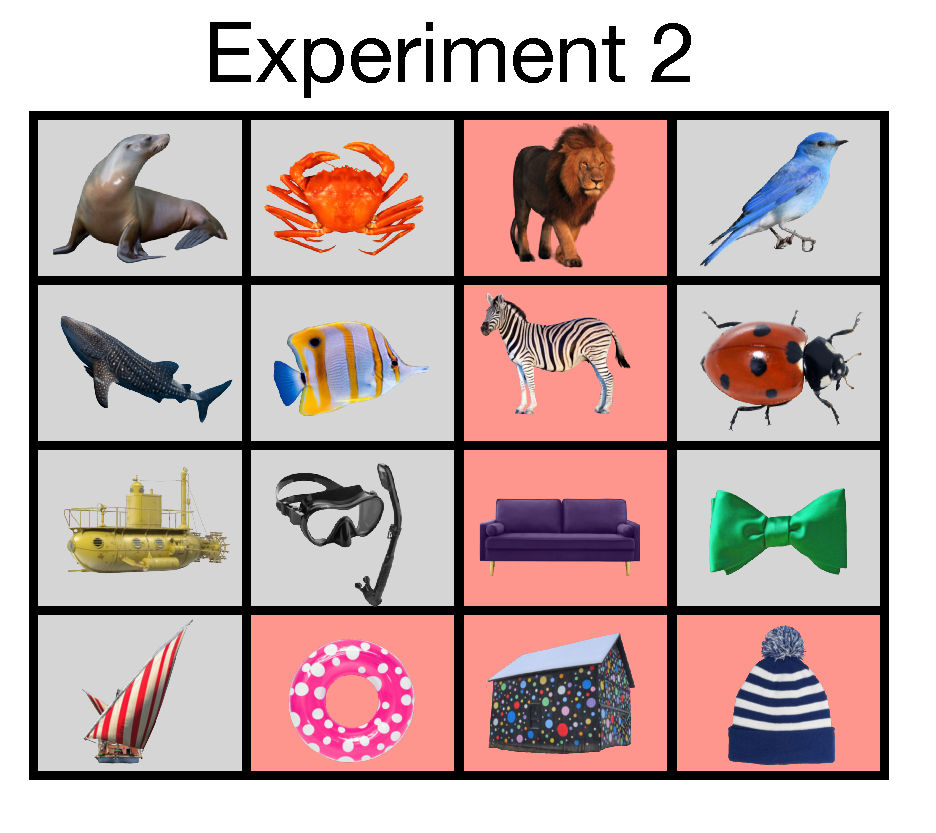
\includegraphics[width=0.4
    \textwidth]{figures/FigureS1.pdf}
    \caption{The full set of stimuli used in experiment two, which differed along four dimensions: pattern (solid or patterned), location (land or sea), animacy (animal or object), and size (small or large). Six images were again sampled to be shown in each round (with an example in red).}
    \label{fig:suppFig1}
\end{figure*}

 % Figure S2
  \clearpage
\begin{figure*}[h]
    \centering
    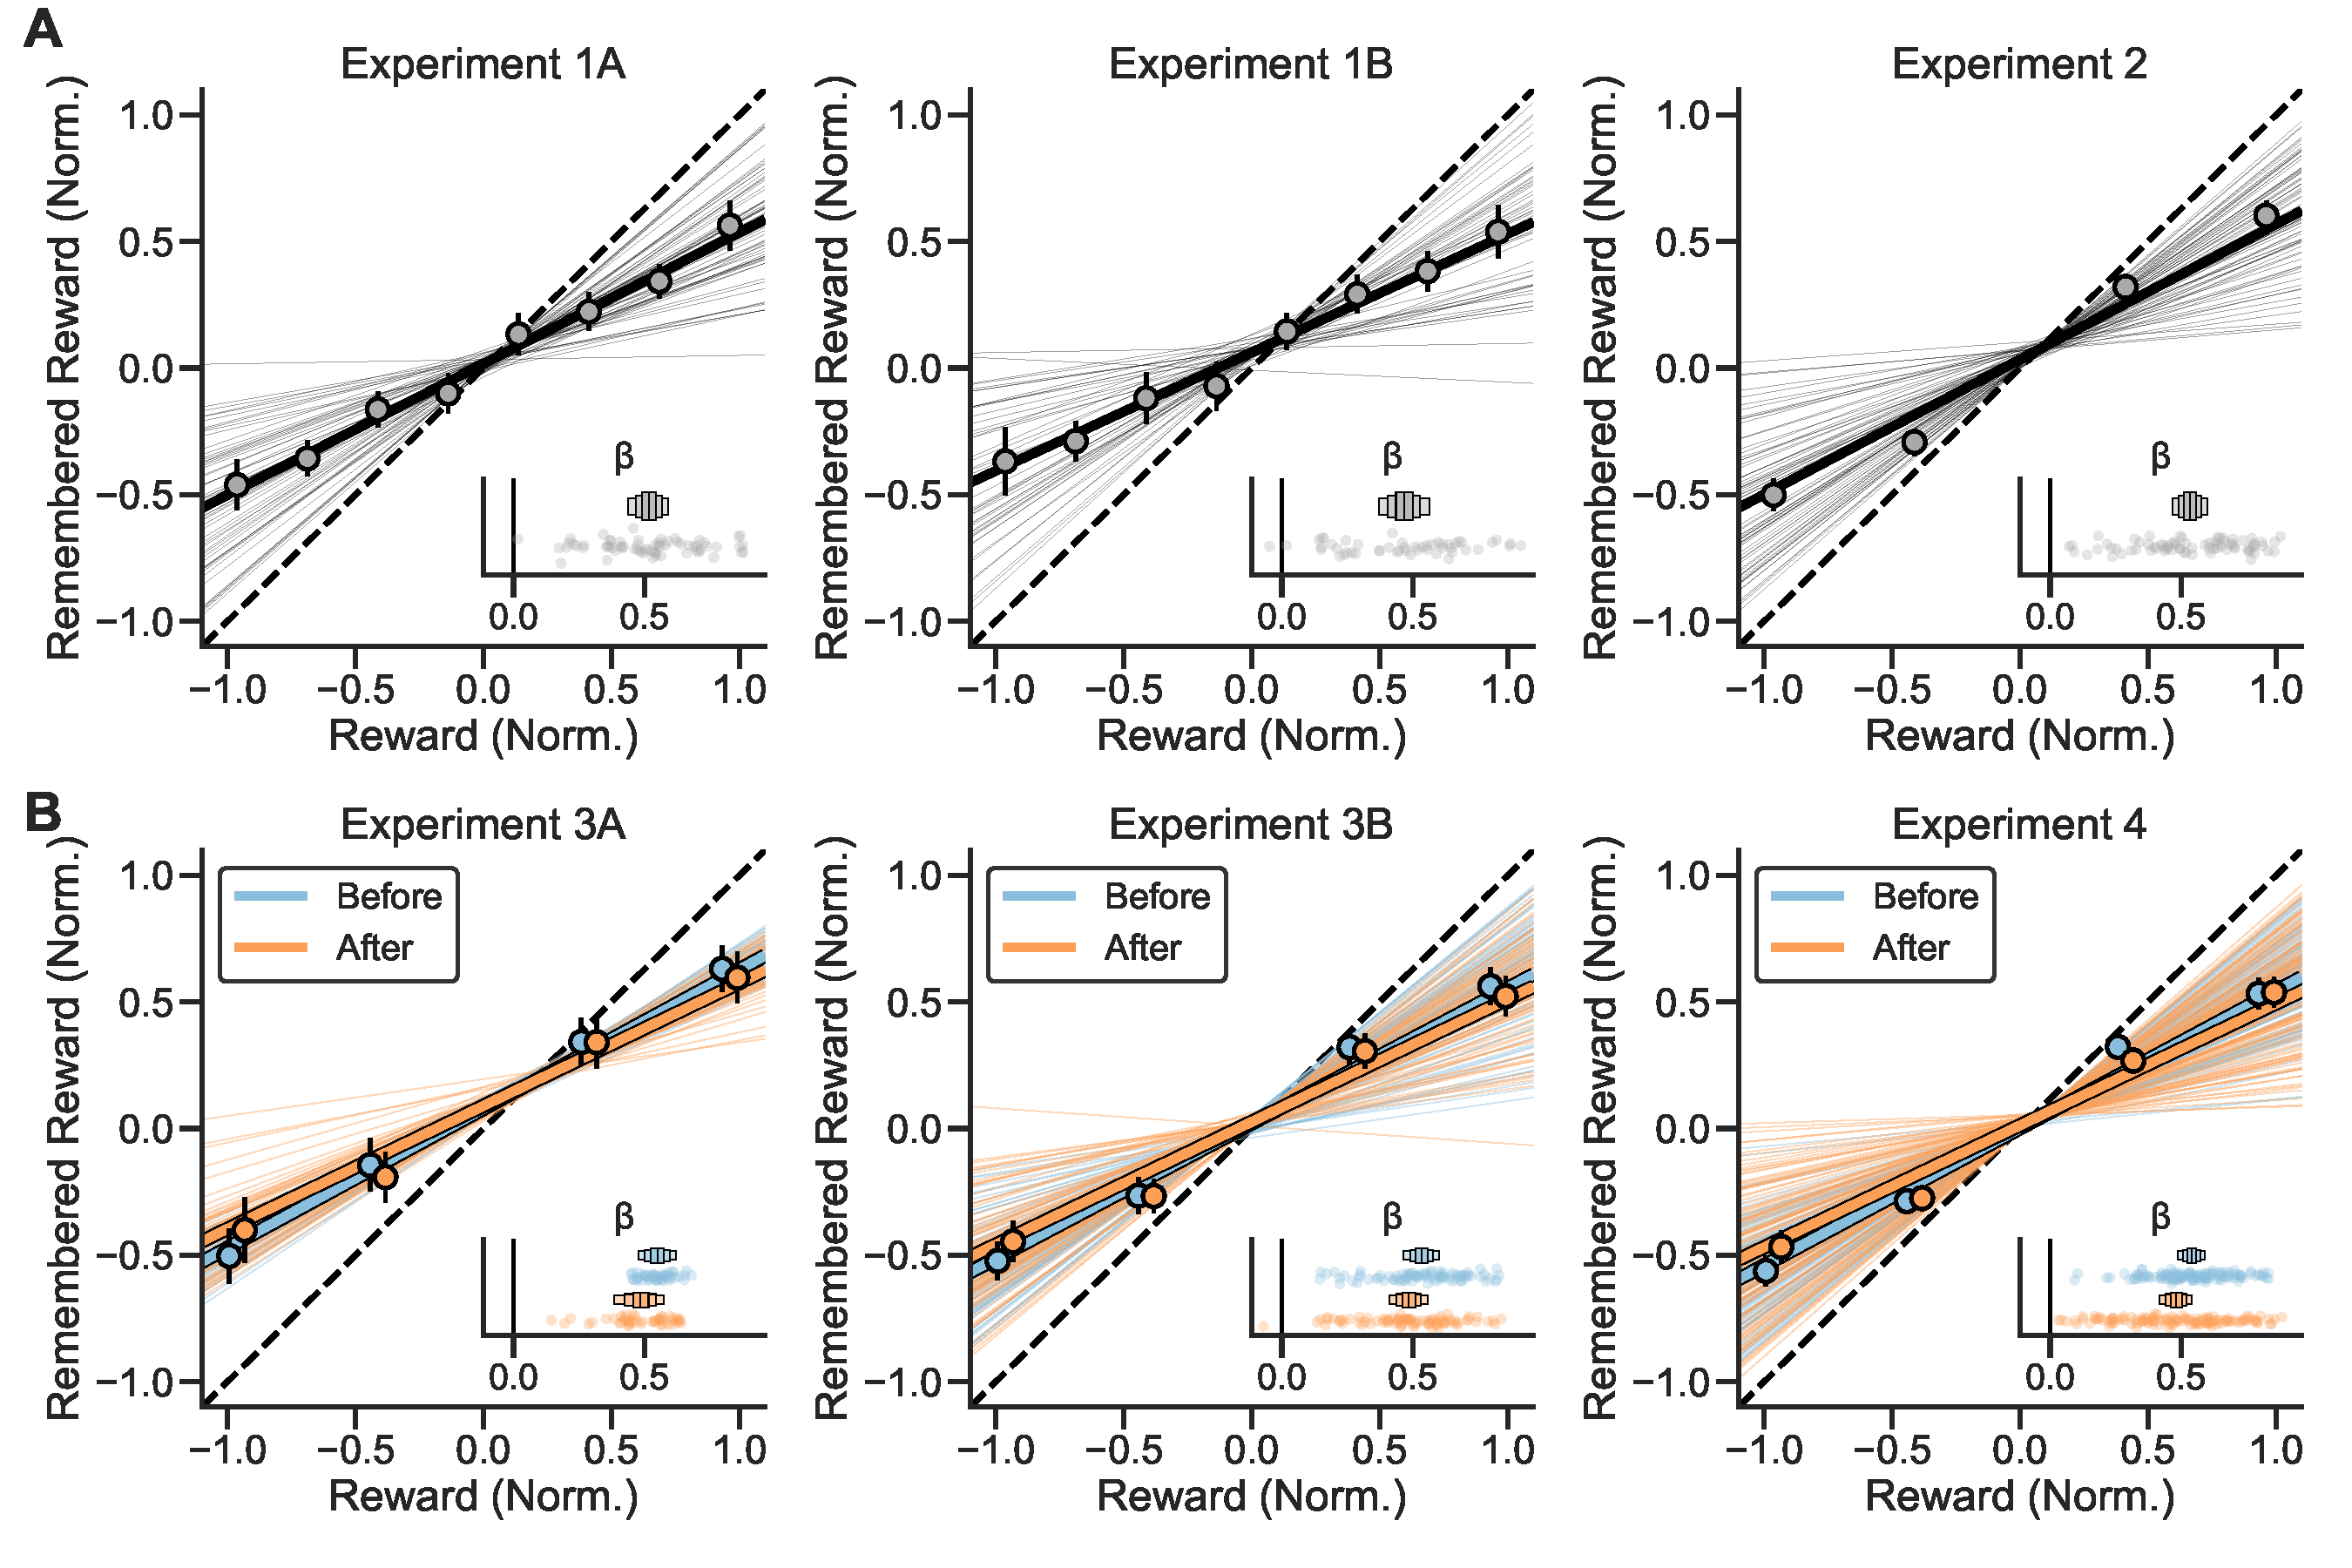
\includegraphics[width=1
    \textwidth]{figures/FigureS2.pdf}
    \caption{Lag-conditional response probability (CRP) curves demonstrating the classic contiguity effect (in which items encoded closer in time to one another are recalled more closely together in time \cite{kahanaFoundationsHumanMemory2012}) in free recall data for experiments one and two (\textbf{A}) and experiments three and four (\textbf{B}). Lines represent group-level averages and bands represent 95\% CIs.}
    \label{fig:suppFig2}
\end{figure*}

 % Figure S3
 \clearpage
\begin{figure*}[h]
    \centering
    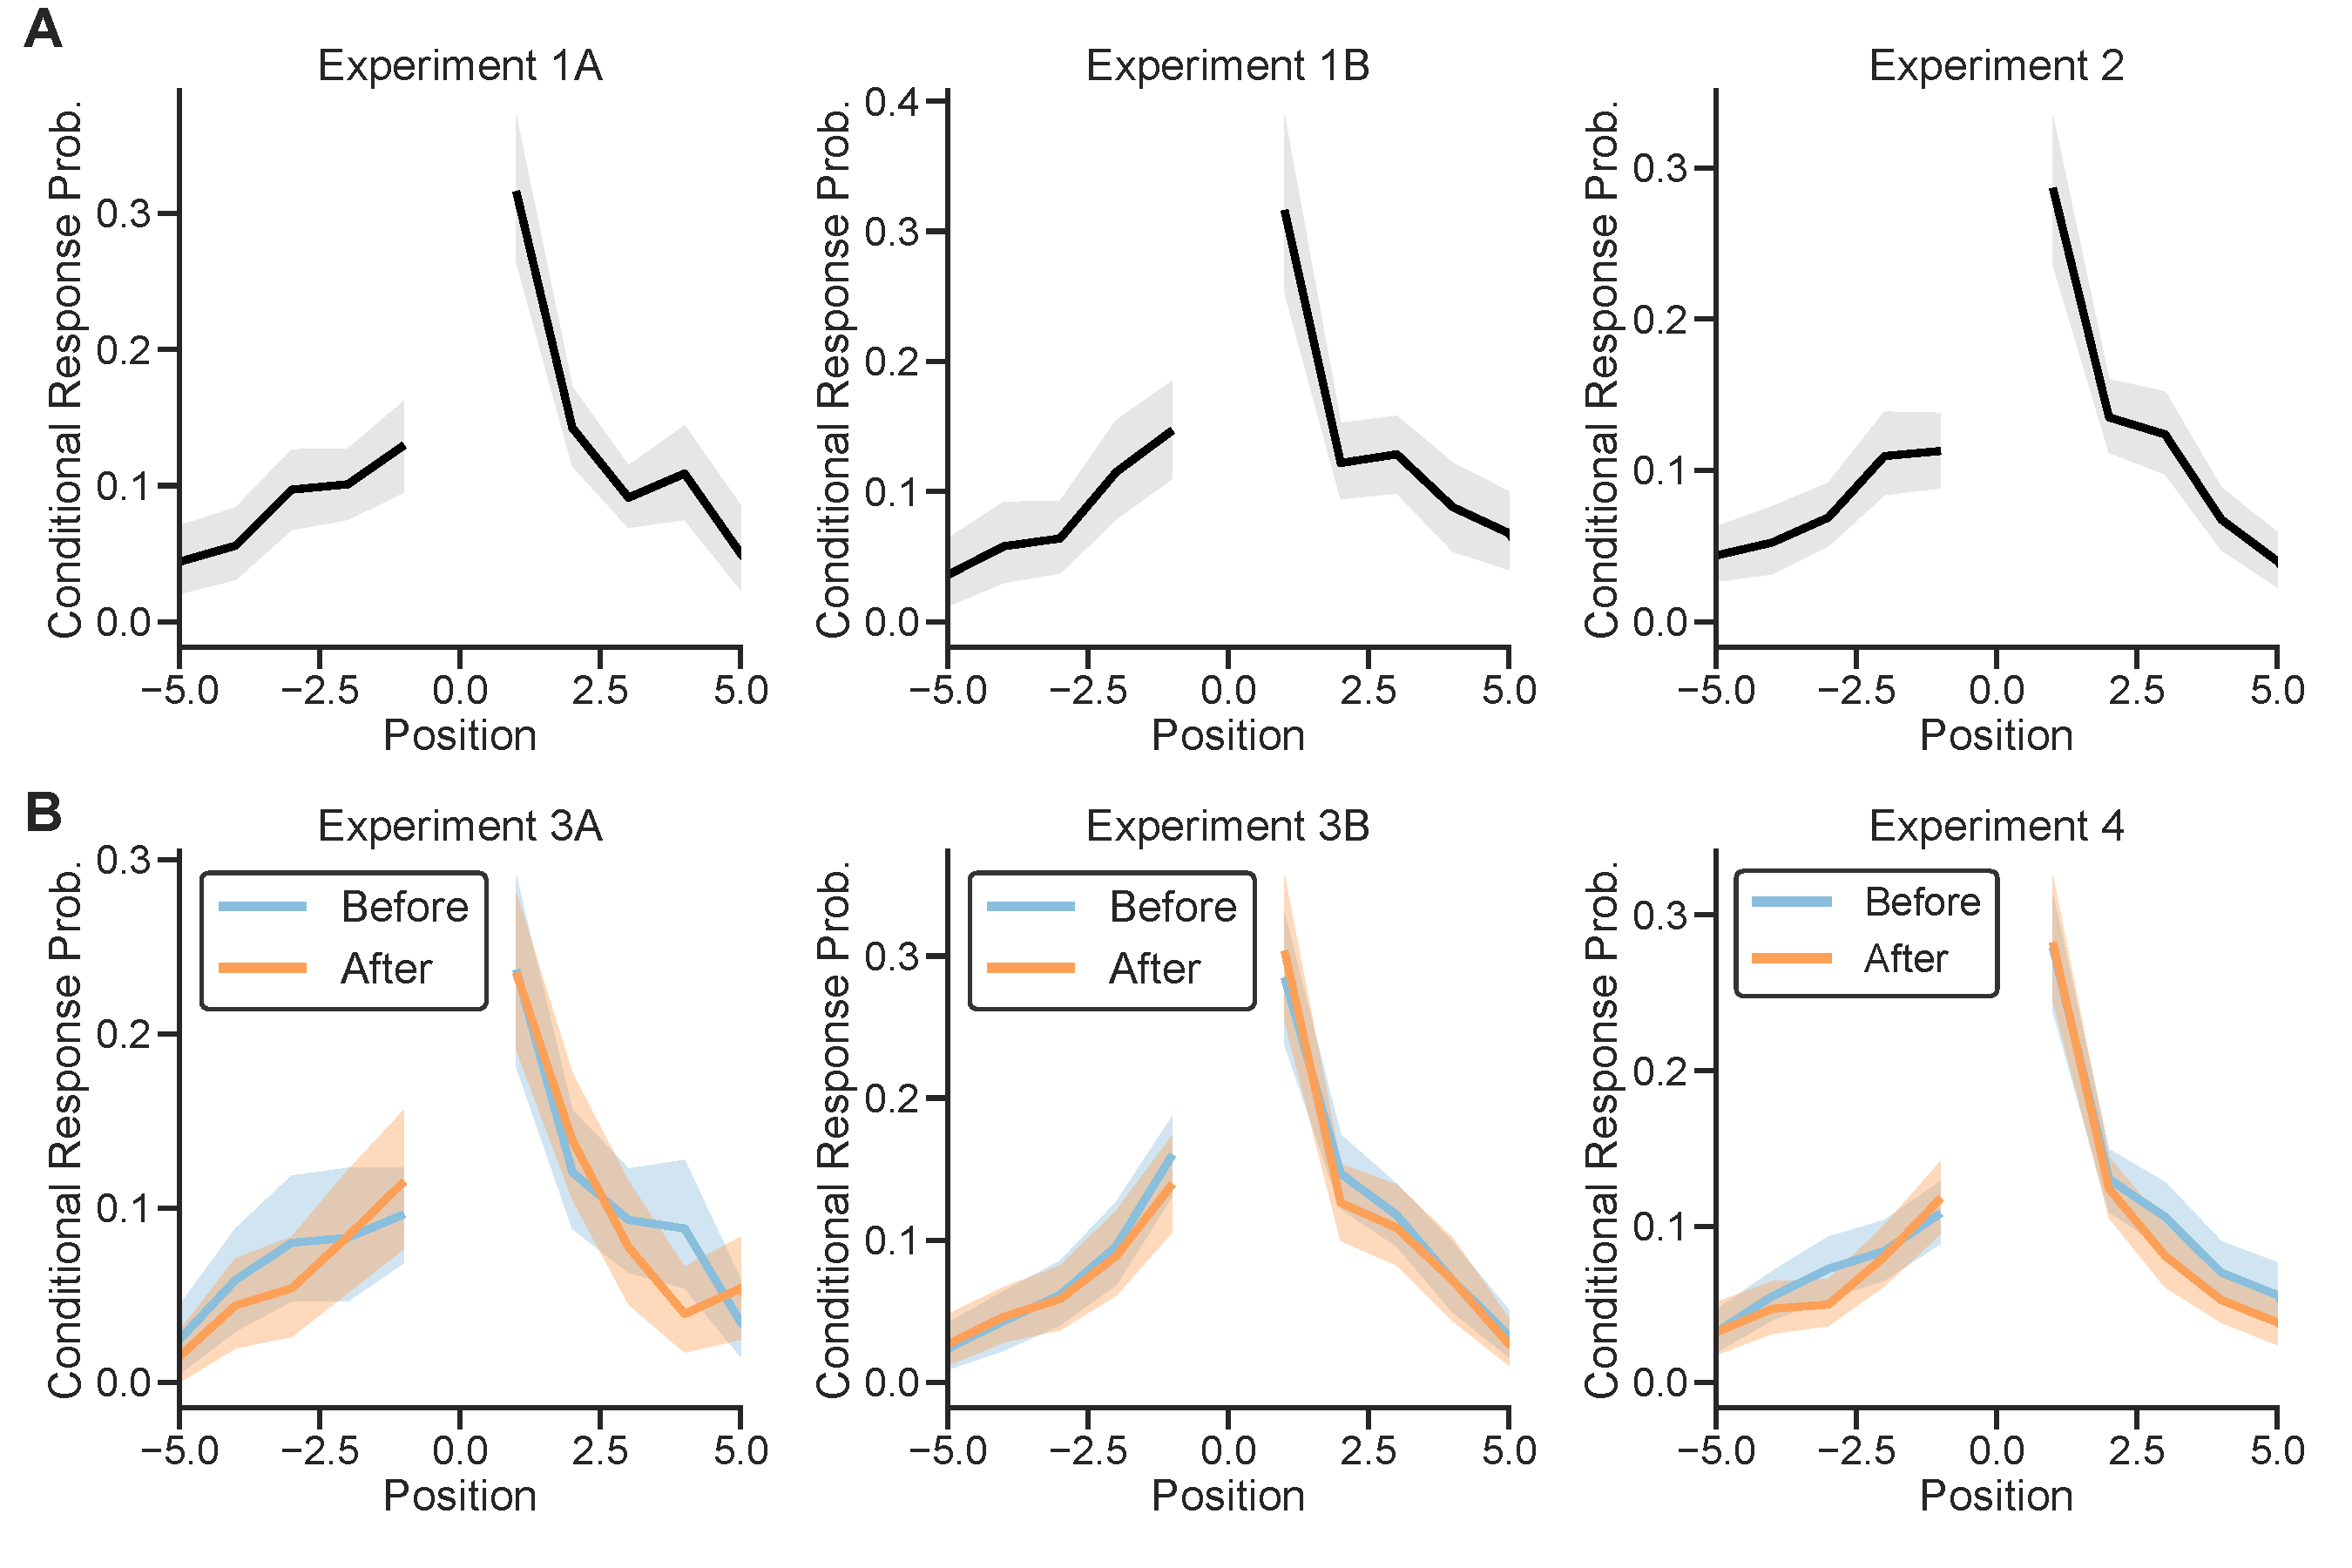
\includegraphics[width=1
    \textwidth]{figures/FigureS3.pdf}
    \caption{Participants' remembered reward reported for each item during the reward memory portion of the memory phase for experiments one and two (\textbf{A}) and experiments three and four (\textbf{B}). The remembered reward for each item is plotted as a function of the item's true associated reward. Large lines represent the group-level fit of a mixed-effects regression, with individual subject fits plotted as smaller lines. Points represent group-level averages with standard error. Inlays show fixed and random effects, where boxes represent the fixed effects posterior distribution with horizontal lines representing the mean and boxes representing 50\%, 80\%, and 95\% HDIs. Points represent random effects slopes for each subject.}
    \label{fig:suppFig3}
\end{figure*}

\end{document}
